\documentclass[color]{tumphthesis}



\usepackage{graphicx}       % Pachet pentru imagini
\usepackage{caption}        % Legende pentru figuri
\usepackage{subcaption}     % Subfiguri pentru matricea de imagini
\usepackage{natbib}
\usepackage{epigraph}
\usepackage{lipsum}
\usepackage{glossaries}
\usepackage[romanian]{babel}
\usepackage[hyphens]{url}

\usepackage{listings}        % Suport pentru afisarea codului sursă
\usepackage{xcolor}          % Pentru culori personalizate în cod

% Definirea stilului pentru cod sursă
\lstdefinestyle{arduino}{
    language=C++,                   % Limba folosită (C++ pentru Arduino)
    basicstyle=\ttfamily\small,     % Font monospaced mic
    keywordstyle=\color{blue},      % Cuvinte cheie în albastru
    commentstyle=\color{gray},      % Comentarii în gri
    stringstyle=\color{green!70!black}, % Șiruri de caractere verzi
    numberstyle=\tiny\color{gray},  % Numerele de linie în gri mic
    numbers=left,                   % Numerotare pe marginea stângă
    stepnumber=1,                    % Fiecare linie numerotată
    showstringspaces=false,         % Nu arată spațiile în șiruri
    tabsize=2,                      % Dimensiunea tab-urilor
    breaklines=true,                % Rupe liniile prea lungi
    breakatwhitespace=false,        % Rupe liniile chiar și la cuvinte
    frame=lines,                    % Linie de cadru deasupra și dedesubt
}


%in lco te chapter e capitol
%\renewcommand{\chaptername}{Capitolul}

%se creeaza lista de abrevieri
\renewcommand{\glossarysection}[2][]{}
\makenoidxglossaries
\newacronym{iot}{IoT}{Internet of Things}

\newacronym{dc}{DC}{Direct Current - Curent Continuu}

\newacronym{pwm}{PWM}{Pulse Width Modulation - Modulație în lățime de puls} % Modulație în lățime de puls

\newacronym{led}{LED}{Light Emitting Diode - Diodă emițătoare de lumină}

\newacronym{sg90}{SG90}{Model de servomotor continuu 360°}  

\newacronym{mah}{mAh}{Miliamperi-oră - unitate de măsură a capacității bateriei}

\newacronym{atmega}{ATmega328P}{Microcontroler utilizat în placa Arduino UNO}

\newacronym{3d}{3D}{Trei Dimensiuni - Reprezentare tridimensională}


\setlength{\parindent}{0pt}    % Elimină indentarea paragrafelor
\setlength{\parskip}{10pt}     % Adaugă 10pt spațiu între paragrafe

\thesistitle
{Inovații în Prepararea Ceaiului: Controlul Infuziei prin Microcontroller}
{Controlul Infuziei prin Microcontroller}
\thesisauthor{Denisa-Maria GOREA}{Denisa-Maria GOREA}
\thesisdate{2024}{12}{25}
\date{\today}


\begin{document}

\maketitle

\abstractpage
%\clearpage
%\chapter*{Abstract}
%\addcontentsline{toc}{chapter}{\protect Abstract}


Această lucrare prezintă proiectarea și %
implementarea unui sistem automatizat pentru %
prepararea ceaiului, utilizând un %
microcontroler bazat pe ATmega328P. Proiectul %
integrează componente electronice accesibile, %
cum ar fi servo motoare, LED-uri, butoane %
și o sursă de alimentare portabilă, %
pentru a demonstra aplicabilitatea %
tehnologiilor moderne în automatizarea %
activităților cotidiene.  

Sistemul controlează un un braț miniatural, %
capabil să ridice %
și să coboare un pliculeț de ceai %
într-o ceașcă, în funcție de un %
temporizator programabil. Controlul motorului %
este realizat prin semnale PWM, asigurând %
o mișcare precisă și repetabilă. %
De asemenea, designul modular permite %
extinderea ulterioară a funcționalităților, %
inclusiv integrarea unor senzori %
suplimentari pentru monitorizarea %
temperaturii și greutății.  

Lucrarea oferă o analiză detaliată %
a configurației componentelor electronice, %
a principiilor de funcționare și a %
etapelor de implementare. Sunt discutate %
problemele întâmpinate pe parcursul %
realizării proiectului, precum și %
soluțiile adoptate pentru  %
performanței sistemului.  

Rezultatele experimentale confirmă %
fezabilitatea soluției propuse și relevă %
oportunități pentru îmbunătățiri viitoare, %
inclusiv adăugarea conectivității wireless %
pentru control de la distanță. Proiectul %
demonstrează utilitatea practică a unui %
sistem simplu și eficient, aplicabil %
atât în scopuri educaționale, cât și %
ca soluție pentru optimizarea %
proceselor casnice.  


\tableofcontents


%se printeaza lista de abrevieri cu titlu pus de mine 
\abreviations
\printnoidxglossaries

\mainmatter\setcounter{page}{1}
\chapter{Introducere}
\label{chap:intro} 

\section{Justificarea abordării temei}
\label{sec:justification}

Proiectul propus are ca obiectiv dezvoltarea %
unui sistem automatizat pentru prepararea %
ceaiului, utilizând o mini-macara %
controlată printr-un microcontroler ATmega328P %
cu chip CH340G. Alegerea acestei teme este %
justificată de dorința de a demonstra %
aplicabilitatea tehnologiilor moderne de %
automatizare în activități casnice obișnuite. %

Proiectul ilustrează cum un proces %
cotidian poate fi optimizat prin %
integrarea soluțiilor bazate pe \gls{iot} %
și control automatizat. %

Automatizarea procesului de preparare a %
ceaiului oferă un exemplu concret al %
aplicabilității tehnologiilor inteligente, %
care pot simplifica sarcinile zilnice, %
economisind timp și resurse. Această %
abordare contribuie la promovarea %
utilizării microcontrolerelor accesibile %
și ușor de programat, similar cu Arduino, %
pentru dezvoltarea unor soluții %
inovatoare. %

Tema este relevantă și datorită %
interesului crescut pentru dispozitivele %
inteligente și pentru crearea unui mediu %
conectat, unde sarcinile repetitive pot fi %
gestionate eficient cu ajutorul %
automatizării. Astfel, proiectul propune %
o soluție funcțională, ușor de implementat, %
cu aplicabilitate largă în diverse domenii, %
de la uz casnic până la cel educațional. %

Pe lângă beneficiile practice, %
acest proiect a avut un impact semnificativ %
asupra dezvoltării mele personale și %
profesionale. Am dobândit cunoștințe %
extinse despre programarea %
microcontrolerelor, proiectarea %
circuitelor electronice și gestionarea %
proiectelor tehnice. În plus, mi-am %
îmbunătățit abilitățile de rezolvare a %
problemelor și gândirea logică prin %
testarea și optimizarea sistemului. %
Acest proces de învățare practică a %
consolidat înțelegerea conceptelor de %
automatizare și \gls{iot}, oferindu-mi o %
perspectivă mai clară asupra %
potențialului acestor tehnologii.

\section{Importanța și Actualitatea Temei}
\label{sec:importance}

Tema abordată este relevantă în contextul %
actual al tendințelor de automatizare și %
al progresului rapid al tehnologiilor %
integrate. Importanța proiectului rezidă %
în promovarea conceptelor de eficiență %
energetică, confort și control personalizat %
al proceselor domestice. De asemenea, %
creșterea interesului pentru dispozitivele %
inteligente și accesibile face ca acest %
proiect să fie pertinent pentru explorarea %
unor soluții inovatoare la scară redusă. %

Acuitatea temei este subliniată de faptul %
că tehnologiile \gls{iot} devin din ce în ce %
mai prezente în viața cotidiană, iar %
exemplele practice contribuie la adoptarea %
rapidă a acestora în societate. Proiectul %
oferă un exemplu concret și accesibil, %
fiind aplicabil atât în educație, cât și %
în activități casnice. %

\section{Originalitatea și Aplicabilitatea Lucrării}
\label{sec:origsiaplic}

Originalitatea proiectului constă în %
implementarea unui sistem simplu, dar %
eficient, de automatizare, combinând %
componente hardware ușor accesibile cu %
programare software flexibilă. Proiectul %
nu își propune să reinventeze %
automatizarea, ci să aducă o contribuție %
modestă și practică la utilizarea %
tehnologiilor existente. Principiul %
conform căruia progresul tehnologic este %
rezultatul contribuțiilor graduale și %
al îmbunătățirii continue a soluțiilor %
existente constituie baza acestei lucrări. %

Deși nu îmi propun să aduc inovații %
radicale, valoarea proiectului constă în %
adaptarea și integrarea inteligentă a %
tehnologiilor moderne, demonstrând modul %
în care acestea pot fi utilizate pentru %
optimizarea proceselor cotidiene. %

Proiectul demonstrează cum inovațiile %
mici, dar bine gândite, pot îmbunătăți %
procesele cotidiene și pot servi drept %
bază pentru dezvoltări viitoare. Prin %
utilizarea platformei Arduino sau a %
componentelor similare, lucrarea permite %
adaptări și extinderi ulterioare, putând %
fi ușor personalizată în funcție de %
cerințele utilizatorilor. %

Aplicabilitatea lucrării este vastă, %
putând fi folosită atât în scop educativ, %
pentru învățare și experimentare, cât și %
ca soluție concretă pentru optimizarea %
preparării ceaiului în medii rezidențiale %
sau comerciale. Acest proiect poate %
servi, de asemenea, ca bază pentru %
dezvoltarea unor dispozitive similare %
destinate altor procese automatizate din %
gospodărie. %


% A cool list:
% \begin{enumerate}
% 	\item item 1
% 	\item item 2
% 	\item item 3
% \end{enumerate}

% \begin{figure}
% 	\centering
% 	\includegraphics[width=.5\textwidth]{example-image-duck}
% 	\caption{A cool duck}
% 	\label{fig:figure1}
% \end{figure}



\chapter{Proiectarea și Realizarea Sistemului}
\label{chap:2}

\section{Principiul de Funcționare}

\subsection{Descrierea Funcționării Algoritmului}

Acest algoritm controlează un servo motor %
continuu pentru a gestiona un mecanism %
automatizat de preparare a ceaiului. %
Sistemul include un servo motor care %
bobinează o sfoară, ridicând sau %
coborând un clește ce ține un %
pliculeț de ceai. Utilizatorul poate %
seta durata în care pliculețul de ceai %
rămâne în apă folosind un %
buton albastru. Mai jos sunt descrise %
componentele și funcționalitățile %
principale:

\subsection{Funcționarea Sistemului}

\begin{enumerate}
    \item La pornire, sistemul inițializează %
    \gls{led}-urile și servo-ul în poziția %
    neutră.  

    \item Utilizatorul setează durata de %
    infuzare în minute apăsând %
    butonul albastru, fiecare apăsare %
    adăugând un minut.  

    \item Servo-ul poate fi controlat %
    manual folosind:  
    \begin{itemize}
        \item Butonul alb pentru ridicarea %
        cleștelui (sens orar).  
        \item Butonul roșu pentru coborârea %
        cleștelui (sens antiorar).  
    \end{itemize}

    \item Procesul principal este declanșat %
    prin apăsarea butonului de start, %
    care activează \gls{led}-ul roșu pentru %
    a indica începerea procesului.  

    \item Motorul oscilează inițial pentru %
    calibrare, apoi pliculețul %
    rămâne în apă pentru durata %
    setată, afișând timpul rămas %
    pe consola serială.  

    \item La finalul procesului, cleștele %
    este ridicat automat, iar \gls{led}-ul %
    verde clipeste pentru a semnaliza %
    încheierea operațiunii.  
\end{enumerate}

\subsection{Inițializare Componente}

\begin{itemize}
    \item Se definesc pini pentru \gls{led}-uri, %
    butoane și controlul servo-ului.  

    \item Se configurează intrările și %
    ieșirile în funcția \texttt{setup()}.  

    \item Servo-ul este inițializat într-o %
    poziție neutră (1500 microsecunde).  

    \item \gls{led}-urile sunt setate inițial %
    pentru a indica starea sistemului.  
\end{itemize}

\subsection{Setarea Timpului de Preparare}

\begin{itemize}
    \item \textbf{Butonul albastru (CountButton):} %
    La fiecare apăsare, timpul este %
    incrementat cu un minut.  

    \item \gls{led}-ul alb se aprinde temporar %
    pentru a indica o apăsare validă.  
\end{itemize}

\subsection{Control Manual al Servo-ului}

\begin{itemize}
    \item \textbf{Butonul alb (UpWhiteButton):} %
    Când este apăsat, servo-ul se %
    rotește în sens orar %
    (\gls{pwm} = 1200 microsecunde), ridicând %
    cleștele.  

    \item \textbf{Butonul roșu (DownRedButton):} %
    Când este apăsat, servo-ul se %
    rotește în sens antiorar %
    (\gls{pwm} = 1800 microsecunde), coborând %
    cleștele.  

    \item Când butoanele sunt eliberate, %
    servo-ul este oprit %
    (\gls{pwm} = 1500 microsecunde).  
\end{itemize}

\subsection{Pornirea Procesului Principal}

\begin{itemize}
    \item \textbf{Butonul de start (StartButton):} %
    Inițiază procesul de coborâre a %
    pliculețului de ceai în apă %
    pentru timpul setat.  

    \item \gls{led}-ul roșu se aprinde pentru %
    a indica începerea procesului.  

    \item Servo-ul efectuează o oscilație %
    de 3 cicluri pentru calibrare.  

    \item Procesul principal așteaptă %
    numărul de minute setate %
    (convertit în secunde) și afișează %
    trecerea timpului în consola serială.  

    \item La final, servo-ul ridică %
    cleștele, iar \gls{led}-ul verde %
    clipeste pentru a indica %
    încheierea procesului.  
\end{itemize}

\subsection{Funcții Auxiliare}

\begin{itemize}
    \item \textbf{whiteLed():} Controlează %
    starea \gls{led}-ului alb.  

    \item \textbf{ready\_anim():} Realizează %
    o animație de clipire pentru %
    \gls{led}-ul verde la sfârșitul %
    procesului.  
\end{itemize}


Acest algoritm oferă o soluție automatizată %
și flexibilă pentru prepararea ceaiului, %
permițând utilizatorului să controleze %
durata și mișcarea mecanismului prin %
intermediul butoanelor fizice.




\section{Schema Electrică și Configurația Componentelor}

    \subsection{Schema Electrică}

    \begin{figure}[ht!]
      \centering
      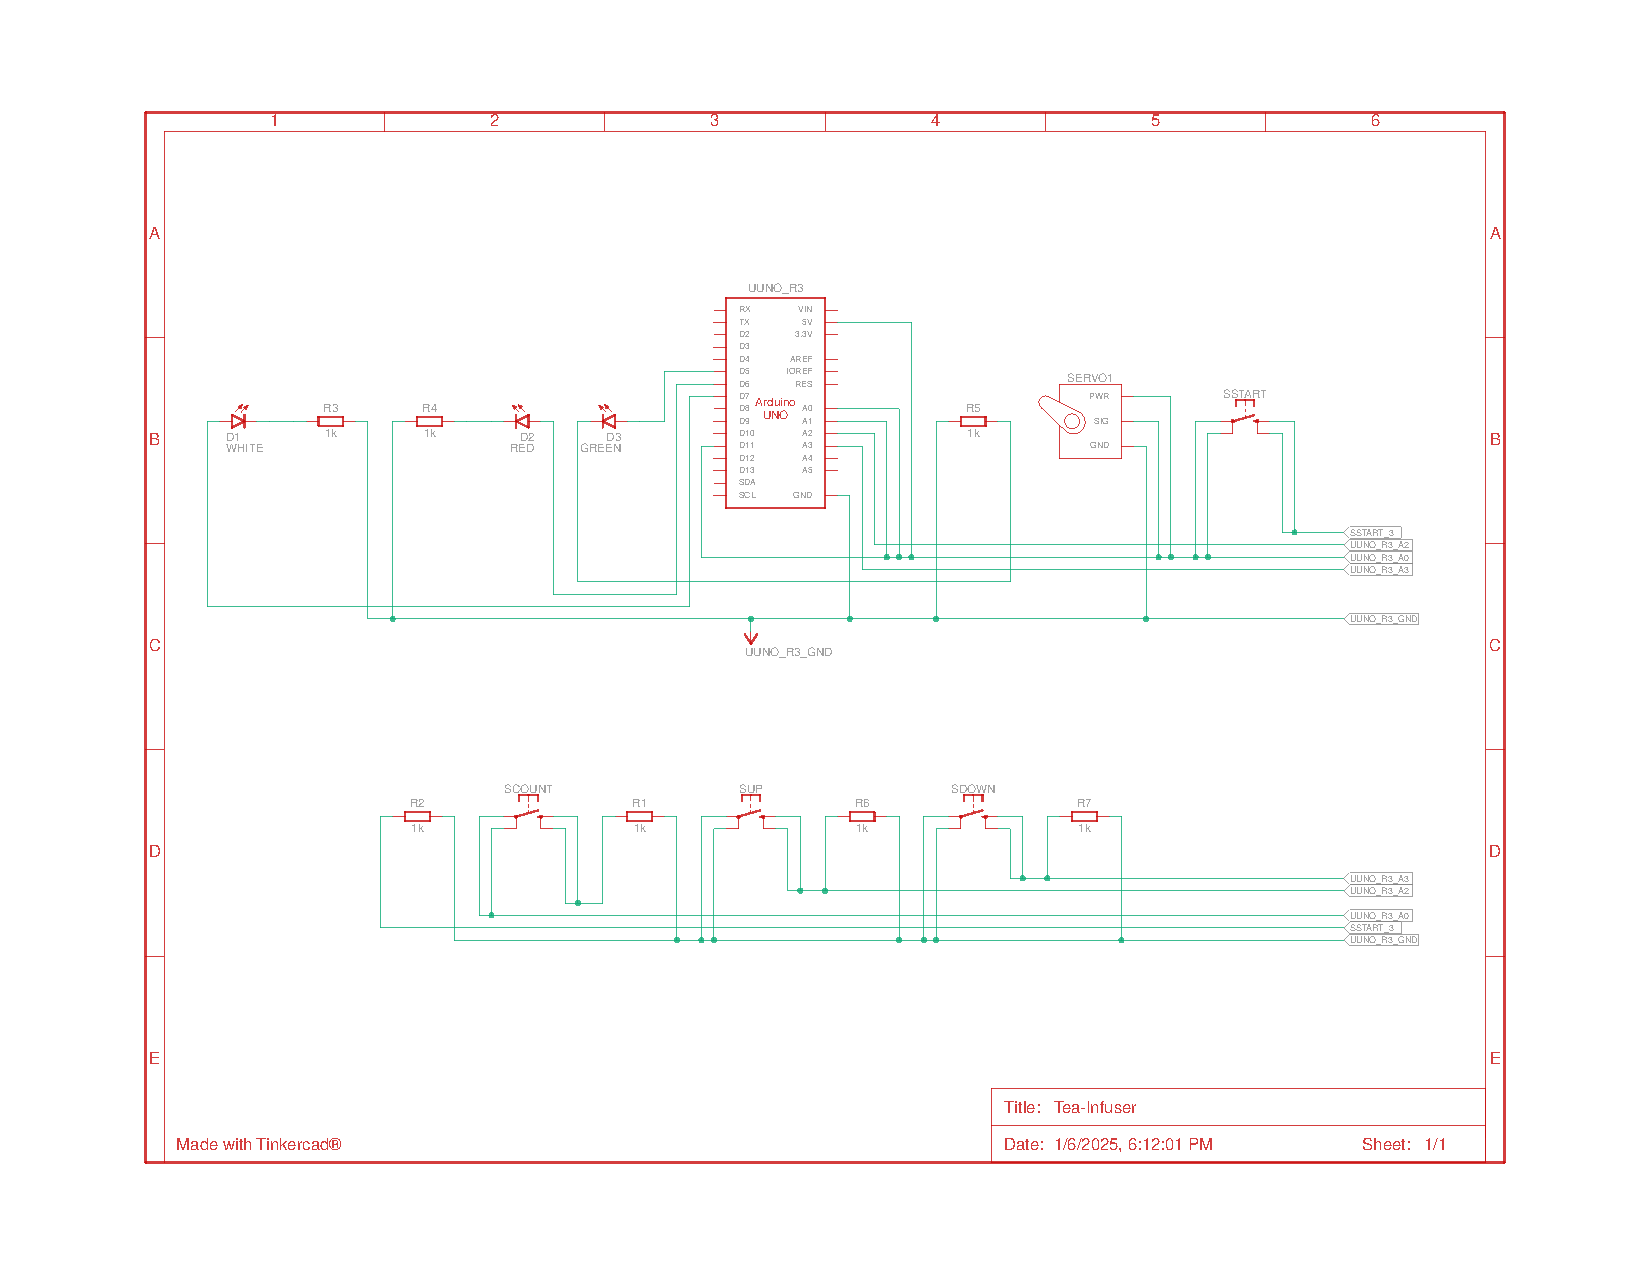
\includegraphics[width=\textwidth]{figures/Schematic.pdf} % Replace 'example.pdf' with your file name
      \caption{Schema Electrică}
      \label{fig:fig1}
    \end{figure}

    \begin{figure}[ht!]
      \centering
      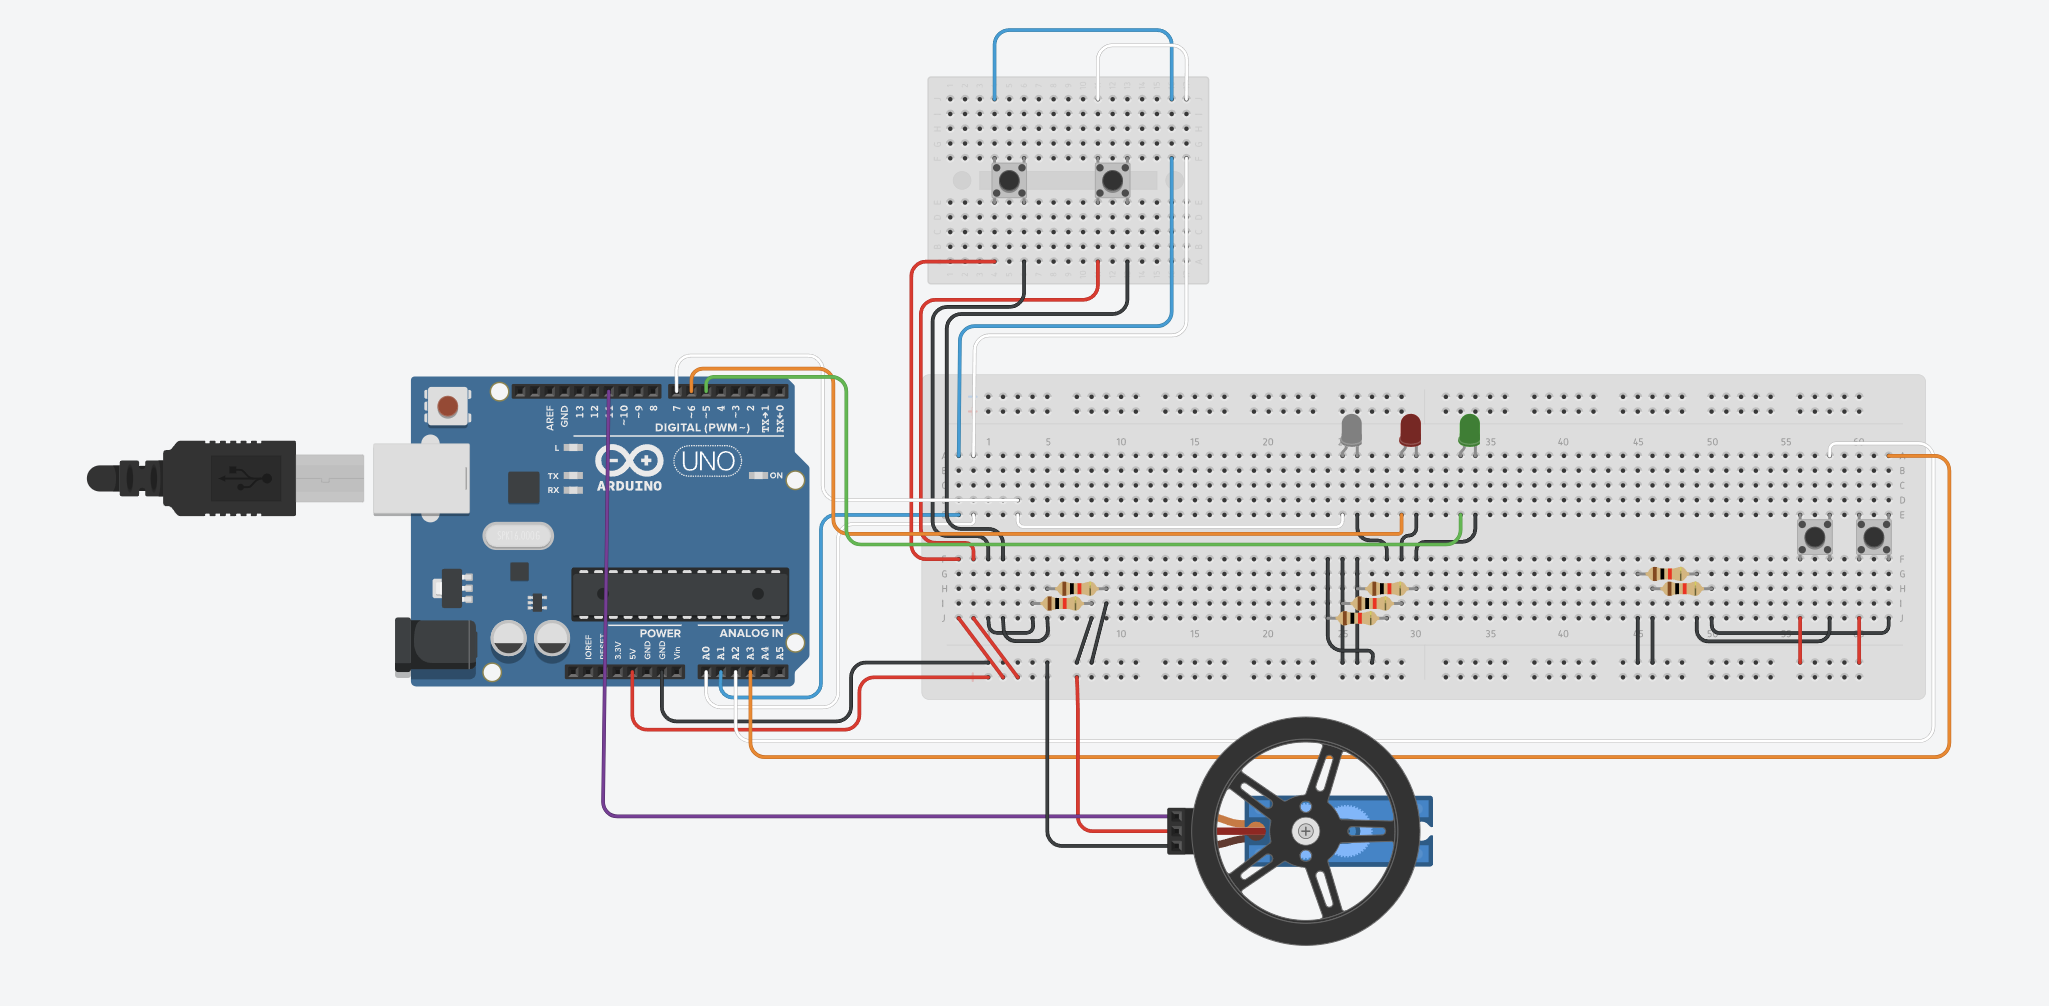
\includegraphics[width=\textwidth]{figures/Circuit.png} % Replace 'example.pdf' with your file name
      \caption{Schemă de Conectare}
      \label{fig:fig2}
    \end{figure}

    \subsection{Configurația Componentelor}
        \begin{itemize}
            \item \textbf{Microcontroler}:  
            Dispozitiv similar cu Arduino UNO R3, %
            bazat pe procesor \gls{atmega} %
            unitatea principală de control. 
            
            \item \textbf{ServoMotor \gls{sg90} 360 grade, continuu}:  
            Utilizat pentru acționarea mecanică a %
            sistemului automatizat.   
    
            \item \textbf{\gls{led}-uri (3 buc.)}:  
              \begin{itemize}
                  \item \gls{led} Verde: Semnalizează abilitatea procesului %
                  de a fi început și terminarea acestuia.  
                  \item \gls{led} Roșu: Semnalizează desfășurarea procesului.  
                  \item \gls{led} Alb: Indică apăsarea de buton pentru a putea %
                  ține cont de numarul de apăsări înregistrate.  
              \end{itemize}
    
            \item \textbf{Butoane (4 buc.)}:  
            \begin{itemize}
              \item Buton Numărător: Incrementează numărul de minute  
              \item Buton Start: Inițiază procesul   
              \item Buton Up: Activează mișcare de ridicare %
              pentru mecanism
              \item Buton Down: Activează mișcare de coborâre %
              pentru mecanism
            \end{itemize}
    
            \item \textbf{Fire de conexiune}:  
            Asigură legăturile electrice între componente.  
    
            \item \textbf{Breadboard}:  
            Utilizat pentru testarea și realizarea conexiunilor provizorii.  
    
            \item \textbf{Baterie externă (2000\gls{mah})}:  
            Baterie externă  cu input 5V/500\gls{mah} și output 5V/1000\gls{mah}, %
            compatibilă cu microcontrolerul și %
            componentele auxiliare pentru funcționarea %
            corectă.   
    \end{itemize}
    



  \section{Probleme Nerezolvate și Motivația Acestora}

    În cadrul proiectului, au fost identificate %
    următoarele probleme nerezolvate, care oferă %
    posibilități de îmbunătățire și dezvoltare %
    ulterioară:
    
    \begin{itemize}
        \item \textbf{Utilizarea senzorilor de greutate:} %
        Sistemul nu include un senzor de greutate %
        pentru a verifica dacă pliculețul de ceai %
        este manipulat corect. Implementarea unui %
        astfel de senzor ar aduce un nivel %
        suplimentar de precizie, dar a fost %
        amânată din cauza constrângerilor de %
        timp și resurse disponibile.  
    
        \item \textbf{Utilizarea senzorilor de poziție:} %
        Lipsa unui senzor de poziție pentru %
        verificarea poziției exacte a %
        pliculețului în timpul manipulării %
        reprezintă o limitare. Un astfel de %
        senzor ar putea îmbunătăți %
        funcționalitatea sistemului prin %
        creșterea acurateței, dar integrarea %
        sa necesită investiții suplimentare %
        în hardware și software.  
    
        \item \textbf{Necesitatea unui senzor de temperatură:} %
        Sistemul nu dispune de un senzor de %
        temperatură pentru monitorizarea apei, %
        ceea ce ar fi util pentru ajustarea %
        automată a timpului de imersiune. %
        Integrarea unui astfel de senzor ar %
        permite optimizarea procesului de %
        preparare a ceaiului, dar această %
        funcționalitate a fost omisă din %
        motive de complexitate și limitări %
        de timp.  
    
        \item \textbf{Conectivitatea cu o aplicație mobilă:} %
        Dispozitivul nu este capabil să %
        comunice cu o aplicație mobilă, %
        deoarece placa utilizată nu dispune %
        de un modul de conectivitate %
        Bluetooth sau Wi-Fi. Această %
        funcționalitate ar fi permis %
        controlul și monitorizarea %
        procesului de la distanță. %
        Integrarea unui modul compatibil %
        necesită componente suplimentare %
        și dezvoltare software avansată.  
    
        \item \textbf{Alimentarea și gestionarea energiei:} %
        Sistemul se bazează pe o baterie %
        externă de 2000\gls{mah}, dar nu a fost %
        testată performanța acesteia pe %
        perioade extinse de utilizare. %
        Monitorizarea consumului și integrarea %
        unei surse de alimentare alternative %
        rămân aspecte de îmbunătățit.  

        \item \textbf{Structura fizică a macaralei:} %
        Structura fizică a macaralei utilizate în acest %
        proiect este una de jucărie, ceea ce limitează aspectul %
        estetic și robustețea acesteia. Utilizarea unei imprimante %
        3D ar fi permis realizarea unui design personalizat, %
        mai atractiv și mai durabil, adaptat cerințelor proiectului.
    \end{itemize}
    
    \bigskip
    
    Problemele identificate în acest proiect %
    subliniază provocările întâmpinate pe parcursul %
    dezvoltării și oferă direcții clare pentru %
    optimizări și îmbunătățiri viitoare.


    

\section{Observații asupra Rezultatelor Obținute}

    Sistemul a demonstrat că poate automatiza %
    procesul de preparare a ceaiului, îndeplinind %
    sarcinile principale pentru care a fost %
    proiectat. Mișcarea mecanismului a fost precisă, %
    iar servo motorul continuu a reușit să %
    înlocuiască eficient motorul \gls{dc} inițial, %
    care nu a avut suficientă putere.  
    
    Testele efectuate au confirmat că dispozitivul %
    funcționează stabil în condiții normale de %
    utilizare. Alimentarea prin baterie a fost %
    suficientă pentru cicluri scurte de operare, %
    dar necesită optimizări pentru utilizarea %
    pe durate mai lungi.  
    
    Butoanele și \gls{led}-urile oferă un sistem de %
    control intuitiv și feedback vizual clar %
    pentru utilizator. Totuși, integrarea unei %
    aplicații mobile ar fi crescut nivelul de %
    utilizare și flexibilitatea dispozitivului.  
    
    În ciuda limitărilor, proiectul a demonstrat %
    fezabilitatea unui sistem automatizat pentru %
    prepararea ceaiului. Rezultatele obținute oferă %
    o bază solidă pentru îmbunătățiri viitoare, %
    atât în ceea ce privește funcționalitatea, %
    cât și aspectul estetic și conectivitatea %
    sistemului.
    





\chapter{Concluzii}

\section{Utilitatea Practică a Lucrării}

Proiectul realizat demonstrează fezabilitatea %
implementării unui sistem automatizat simplu %
și eficient pentru prepararea ceaiului, %
integrând componente electronice accesibile %
și ușor de utilizat. Acesta oferă un %
exemplu concret de aplicare %
a tehnologiilor moderne în optimizarea %
activităților zilnice, evidențiind potențialul %
automatizării în îmbunătățirea confortului %
utilizatorilor.  

Sistemul poate fi folosit atât ca dispozitiv %
practic pentru uz casnic, cât și ca instrument %
educativ pentru învățarea noțiunilor de %
programare, electronice și automatizare. %
Flexibilitatea soluției permite adaptări și %
extinderi viitoare, inclusiv integrarea unor %
senzori suplimentari sau a conectivității %
wireless pentru control la distanță.

\section{Aspecte Economice și Eficiență}

Din punct de vedere economic, sistemul propus %
are un cost de producție redus, datorită %
utilizării unor componente electronice %
comune și ieftine, precum microcontrolerul %
compatibil Arduino, servo motorul continuu %
și \gls{led}-urile. %
 
Acest aspect îl face accesibil atât pentru %
utilizatorii individuali, cât și pentru %
instituțiile educaționale care doresc să %
folosească proiectul în scop didactic.  

Costurile suplimentare pentru îmbunătățiri, %
precum imprimarea \gls{3d} a componentelor %
mecanice sau adăugarea senzorilor de %
greutate, poziție și temperatură, sunt %
moderate și justificate de creșterea %
funcționalității și preciziei sistemului.  

Pe termen lung, dispozitivul poate contribui %
la economisirea timpului utilizatorilor prin %
automatizarea unui proces repetitiv, %
justificând astfel investiția inițială %
prin eficiența obținută.  



\chapter{Bibliografie}

\begin{enumerate}
    \item Arduino. \textit{Arduino Uno Rev3 Pinout Diagram}. %
    Disponibil la: \url{https://docs.arduino.cc/resources/pinouts/A000066-full-pinout.pdf}.

    \item Arduino. \textit{Arduino Uno Rev3 Datasheet}. %
    Disponibil la: \url{https://docs.arduino.cc/resources/datasheets/A000066-datasheet.pdf}.

    \item Microchip. \textit{ATmega328P Datasheet}. %
    Disponibil la: %
    \url{https://ww1.microchip.com/downloads/en/DeviceDoc/ATmega328P_Datasheet.pdf}.

    \item Arduino. \textit{Servo Motors Guide}. %
    Disponibil la: \url{https://docs.arduino.cc/learn/electronics/servo-motors/}.

    \item Harja Gabriel. \textit{Îndrumător Laborator Electronică Digitală}.  

    \item Overleaf. \textit{Learn LaTeX in 30 Minutes}. %
    Disponibil la: \url{https://www.overleaf.com/learn/latex/Learn_LaTeX_in_30_minutes}.

    \item Overleaf. \textit{Table of Contents in LaTeX}. %
    Disponibil la: \url{https://www.overleaf.com/learn/latex/Table_of_contents}.

    \item Overleaf. \textit{Multi-file LaTeX Projects}. %
    Disponibil la: \url{https://www.overleaf.com/learn/latex/Multi-file_LaTeX_projects}.

    \item ISL Products. \textit{Servo Motor Fundamentals}. %
    Disponibil la: \url{https://islproducts.com/design-note/servo-motor-fundamentals/}.

    \item Tinkercad.\textit{Online Circuit Simulation Tool}. %
    Disponibil la:\url{https://www.tinkercad.com/}.
\end{enumerate}


\appendix
\chapter{Codul Sursă}
\label{cha:app1}

\begin{lstlisting}[style=arduino, caption={}]
    #include <Servo.h>
    
    // Definitii pini
    int WhiteLedPin = 5;           // Pin pentru LED-ul alb
    int RedLedPin = 6;             // Pin pentru LED-ul rosu
    int GreenLedPin = 7;           // Pin pentru LED-ul verde
    int CountButtonPin = 15;       // Buton pentru numarare apasari
    int StartButtonPin = 14;       // Buton pentru pornirea procesului
    int UpWhiteButtonPin = 16;     // Buton pentru miscarea motorului in sus
    int DownRedButtonPin = 17;     // Buton pentru miscarea motorului in jos
    int ServoPin = 11;             // Pin de control pentru servo
    
    // Variabile
    Servo myServo;                  // Obiect servo
    int cnt = 0;                     // Contor pentru apasarile butonului
    int min = 0;                     // Durata procesului calculata pe baza apasarilor
    int starePinCountButton = 0;     // Stare pentru debouncing la butonul de numarare
    int starePinStartButton = 0;     // Stare pentru debouncing la butonul de start
    int starePinUpWhiteButton = 0;   // Stare pentru debouncing la butonul alb
    int starePinDownRedButton = 0;   // Stare pentru debouncing la butonul rosu
    int white = 1;                   // Starea LED-ului alb
    int start = 0;                   // Indicator pentru proces in desfasurare
    
    void setup() {
      // Configurare pini
      pinMode(WhiteLedPin, OUTPUT);
      pinMode(RedLedPin, OUTPUT);
      pinMode(GreenLedPin, OUTPUT);
    
      pinMode(CountButtonPin, INPUT);
      pinMode(StartButtonPin, INPUT);
      pinMode(UpWhiteButtonPin, INPUT);
      pinMode(DownRedButtonPin, INPUT);
    
      // Initializare servo
      myServo.attach(ServoPin);             // Ataseaza servo-ul la pin
      myServo.writeMicroseconds(1500);      // Pozitie neutra (stop)
    
      // Stare initiala a LED-urilor
      digitalWrite(WhiteLedPin, HIGH);      // LED-ul alb ON initial
      digitalWrite(GreenLedPin, LOW);
      digitalWrite(RedLedPin, LOW);
    }
    
    void loop() {
      whiteLed();                     // Controleaza starea LED-ului alb
      if (start == 0) counting();     // Numara apasarile butonului cand procesul nu este pornit
    
      // Control pentru UpWhiteButton - Miscare in sens orar cat timp butonul este apasat
      if (digitalRead(UpWhiteButtonPin) == HIGH) {
         starePinUpWhiteButton = 1;              // Stare buton activata
         myServo.writeMicroseconds(1200);       // Misca servo-ul in sens orar
         delay(20);
      }  else {
          starePinUpWhiteButton = 0;
          myServo.writeMicroseconds(1500);      // Opreste servo-ul cand butonul este eliberat
      }
    }
    \end{lstlisting}
    


\chapter{Imagini ale Proiectului Finalizat}

\begin{figure}[h!]
  \centering

  % Rândul 1
  \begin{subfigure}[b]{0.3\textwidth} % 1-a imagine
      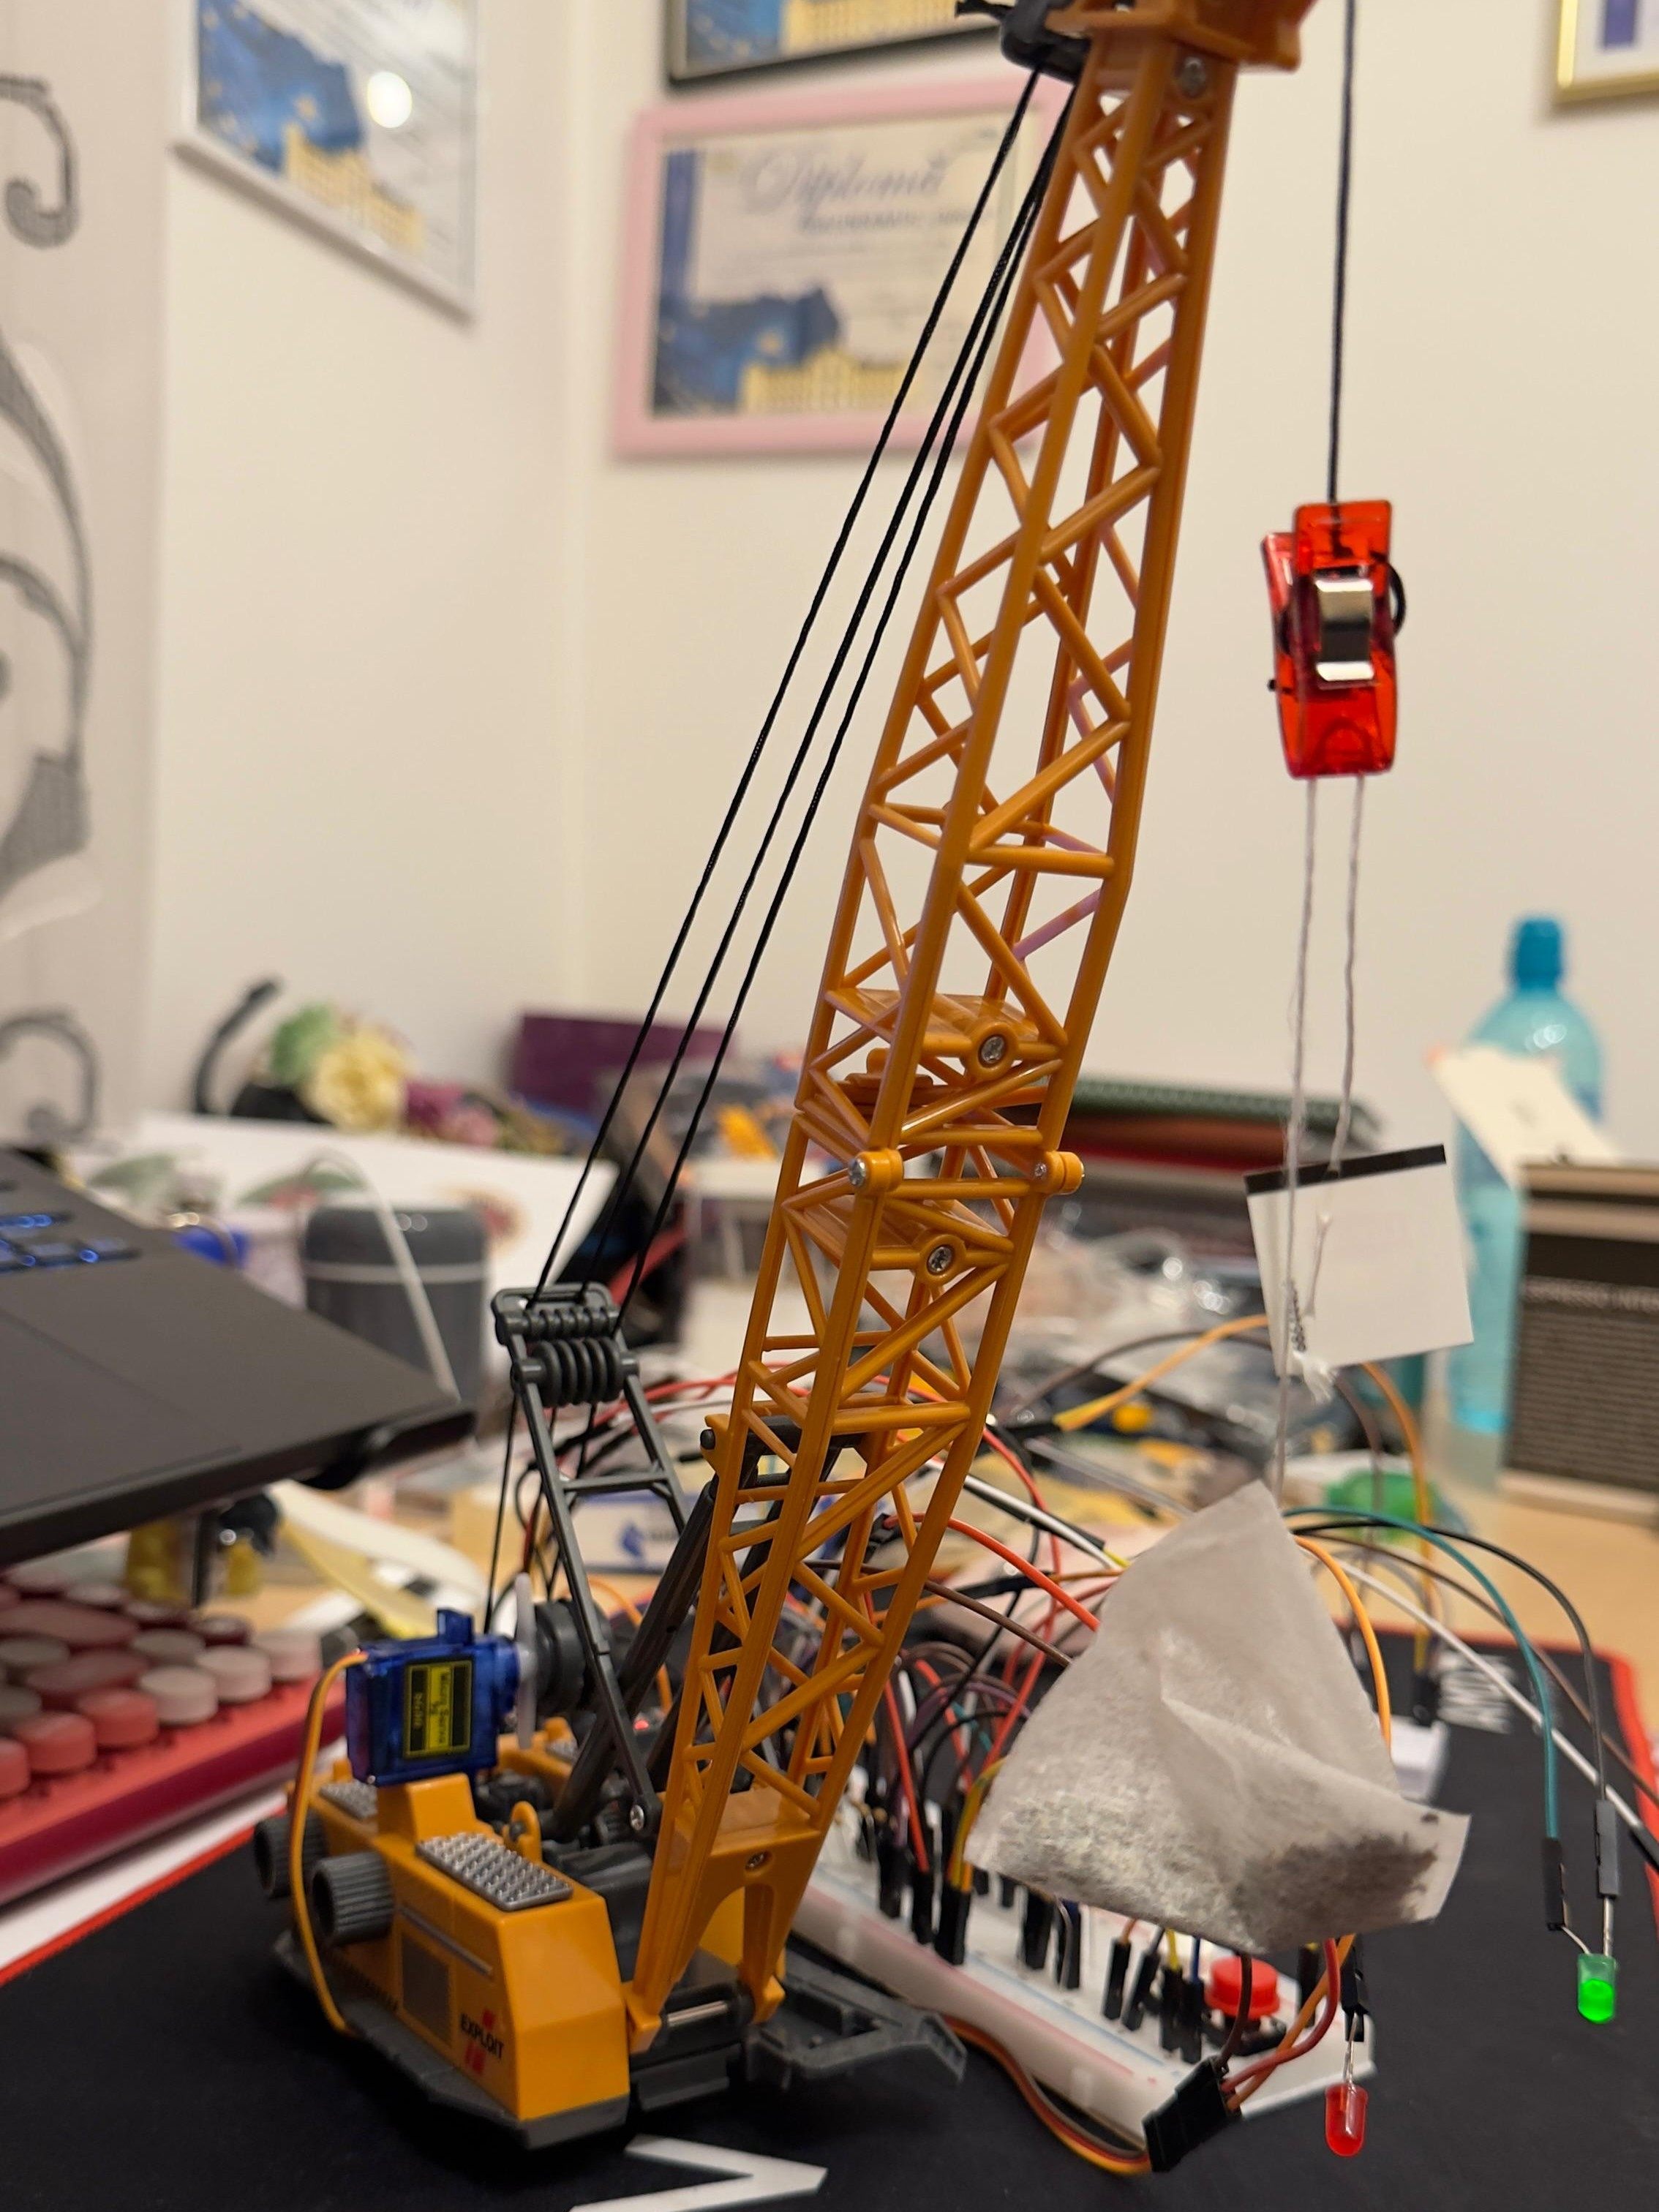
\includegraphics[width=\textwidth]{figures/1.jpg}
      \caption{Macara de jucărie}
  \end{subfigure}
  \hfill
  \begin{subfigure}[b]{0.3\textwidth} % 2-a imagine
      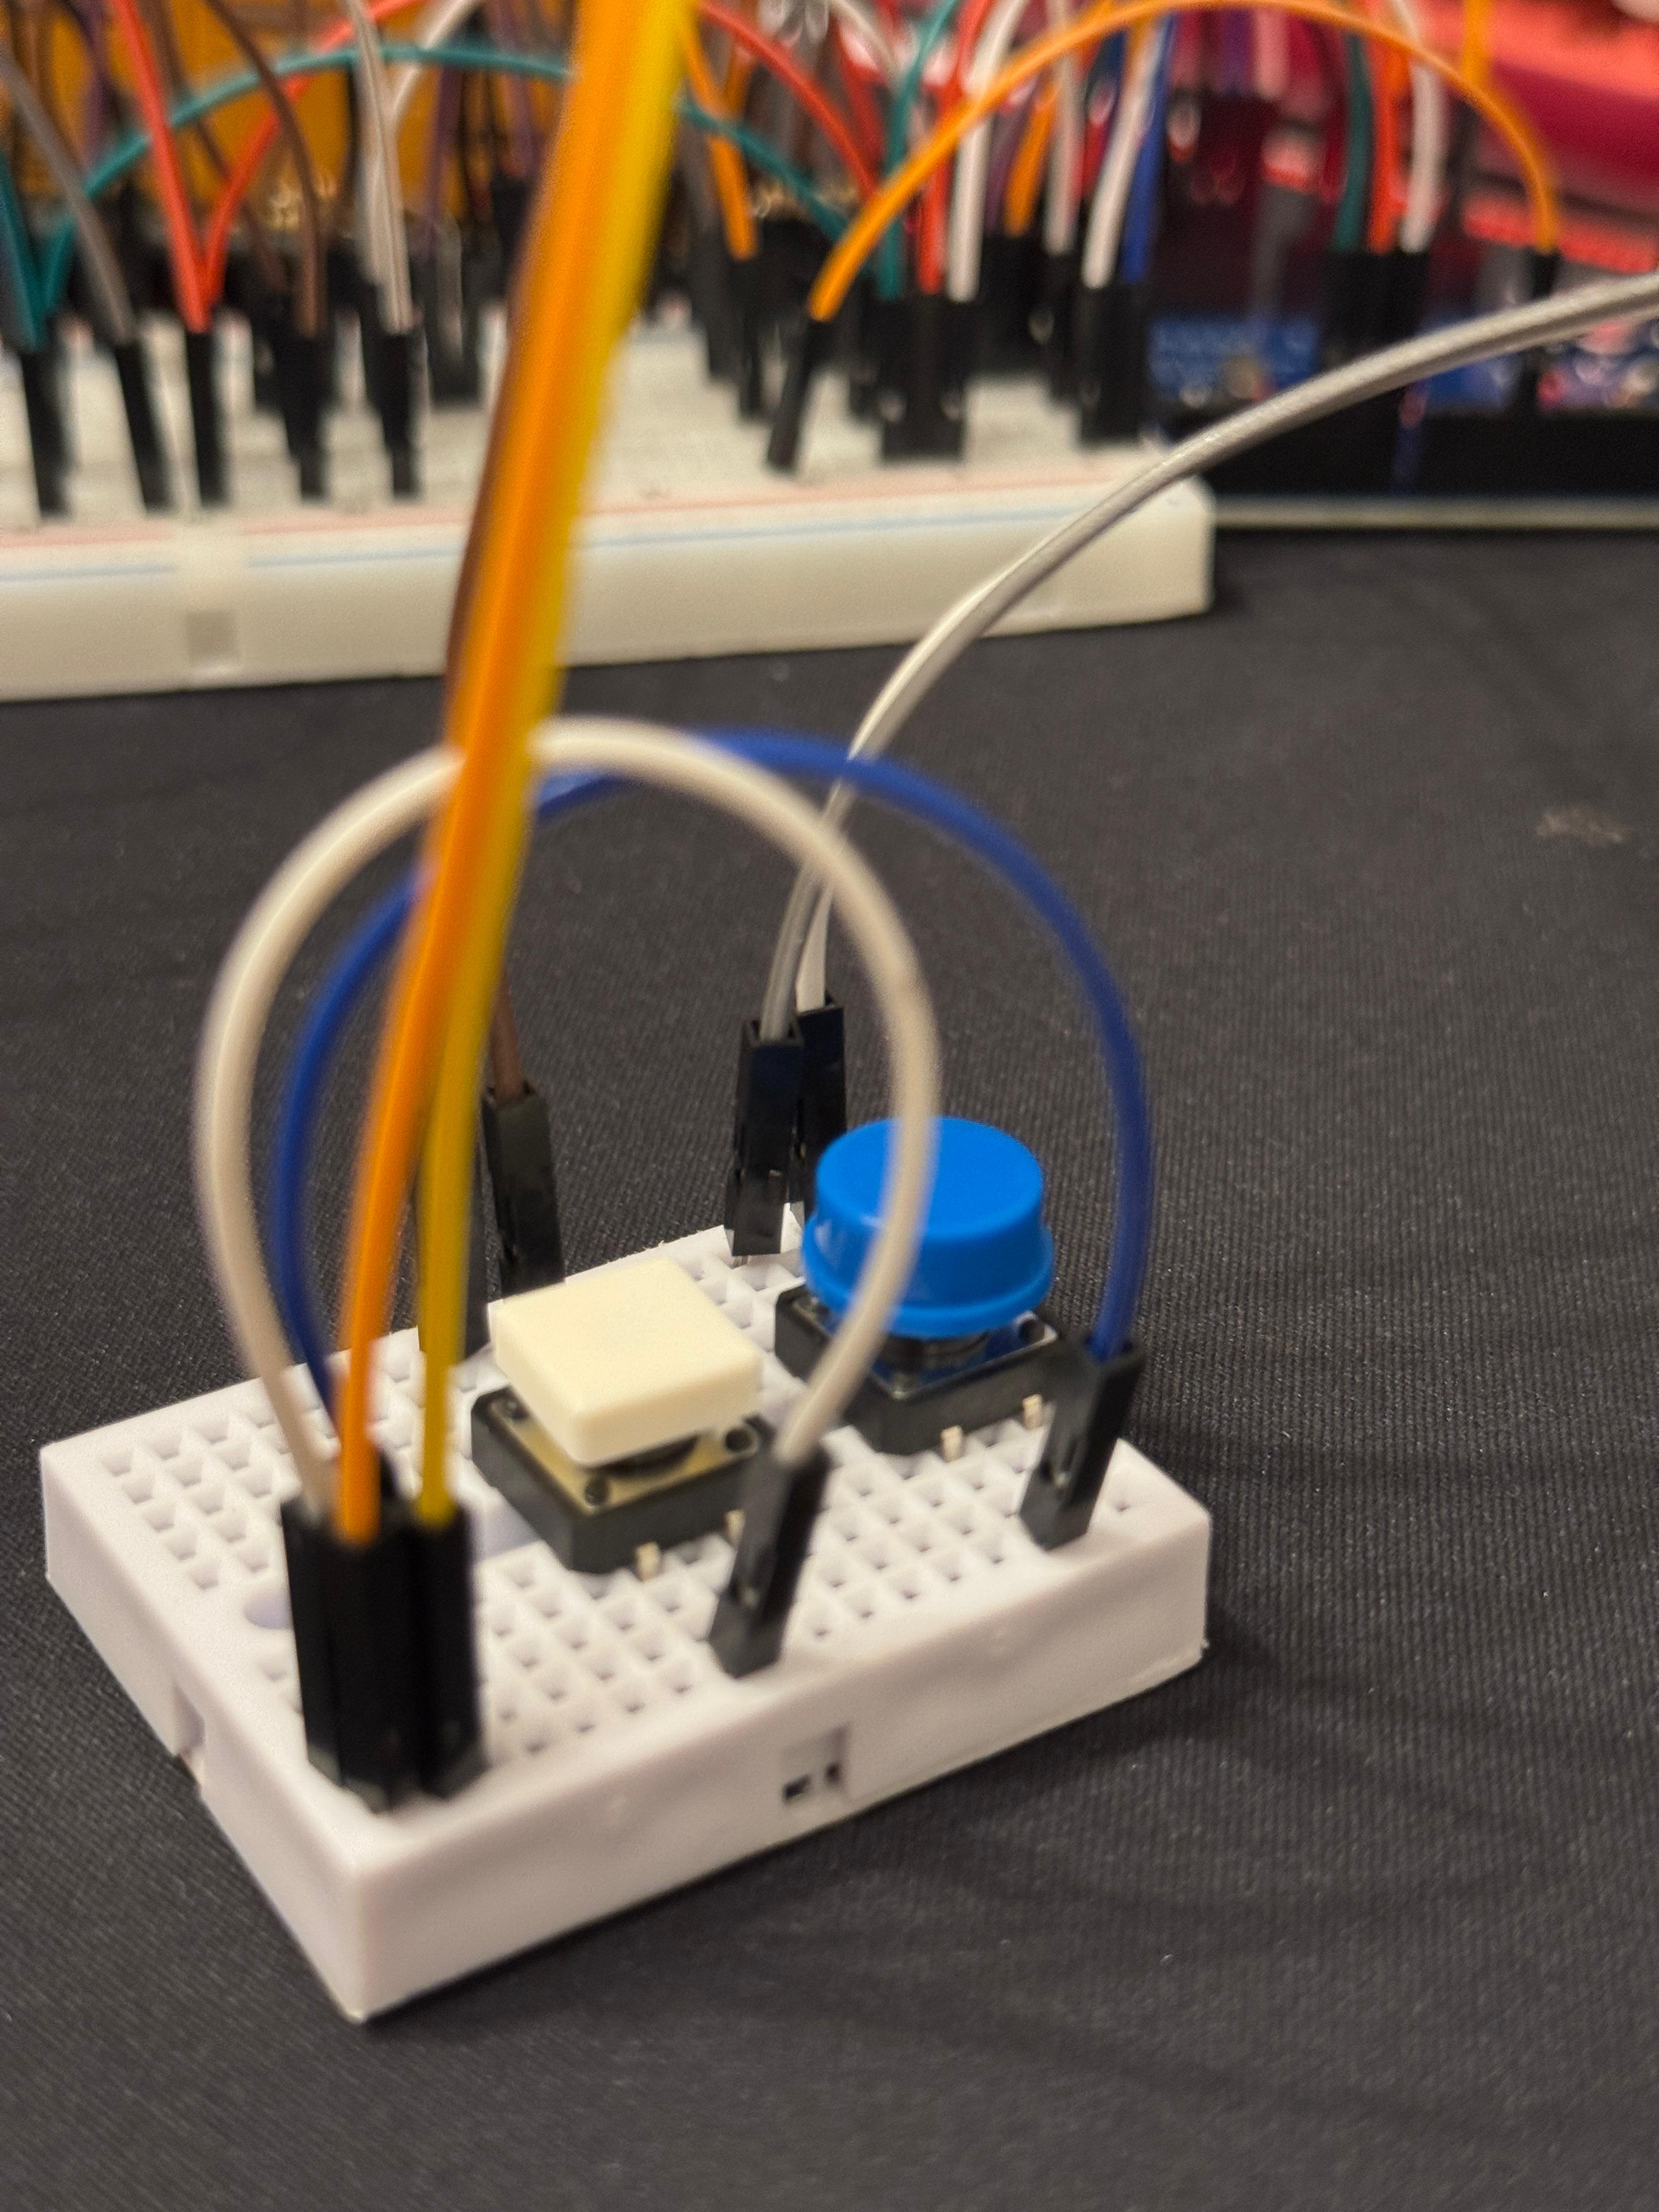
\includegraphics[width=\textwidth]{figures/2.jpg}
      \caption{Butoane Count și Start}
  \end{subfigure}
  \hfill
  \begin{subfigure}[b]{0.3\textwidth} % 3-a imagine
      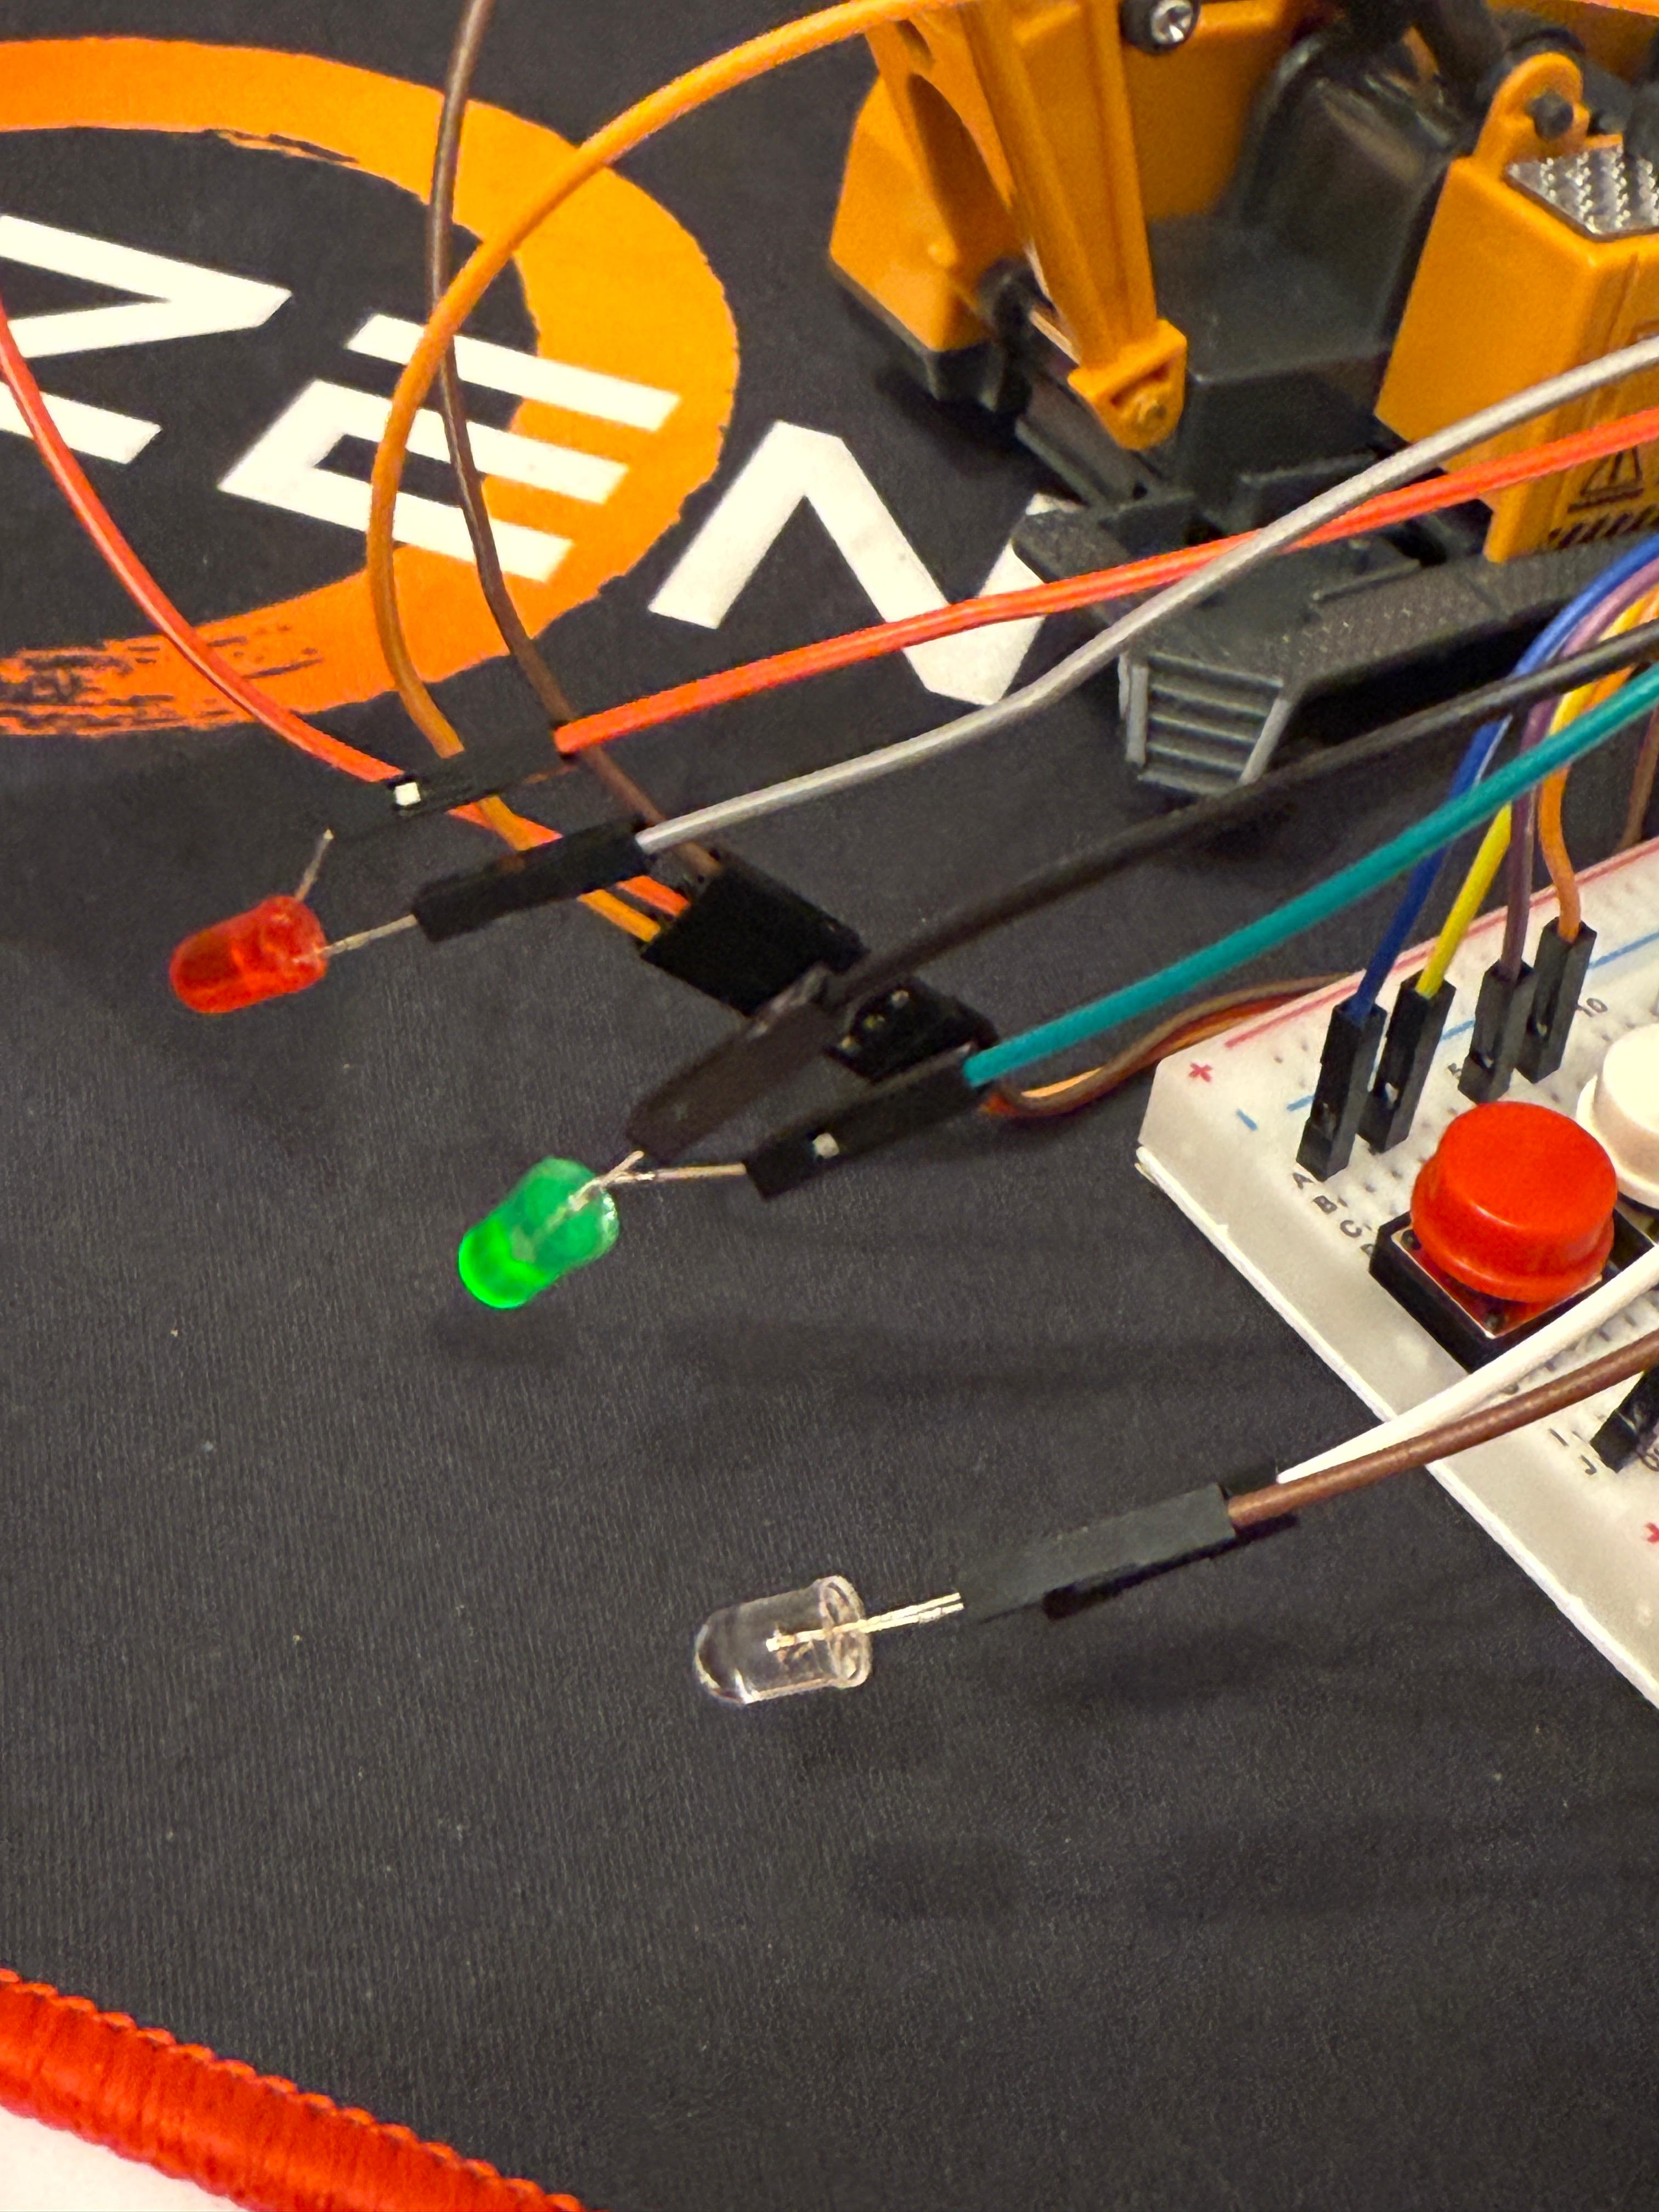
\includegraphics[width=\textwidth]{figures/3.jpg}
      \caption{LED-uri}
  \end{subfigure}

  % Rândul 2
  \begin{subfigure}[b]{0.3\textwidth} % 4-a imagine
      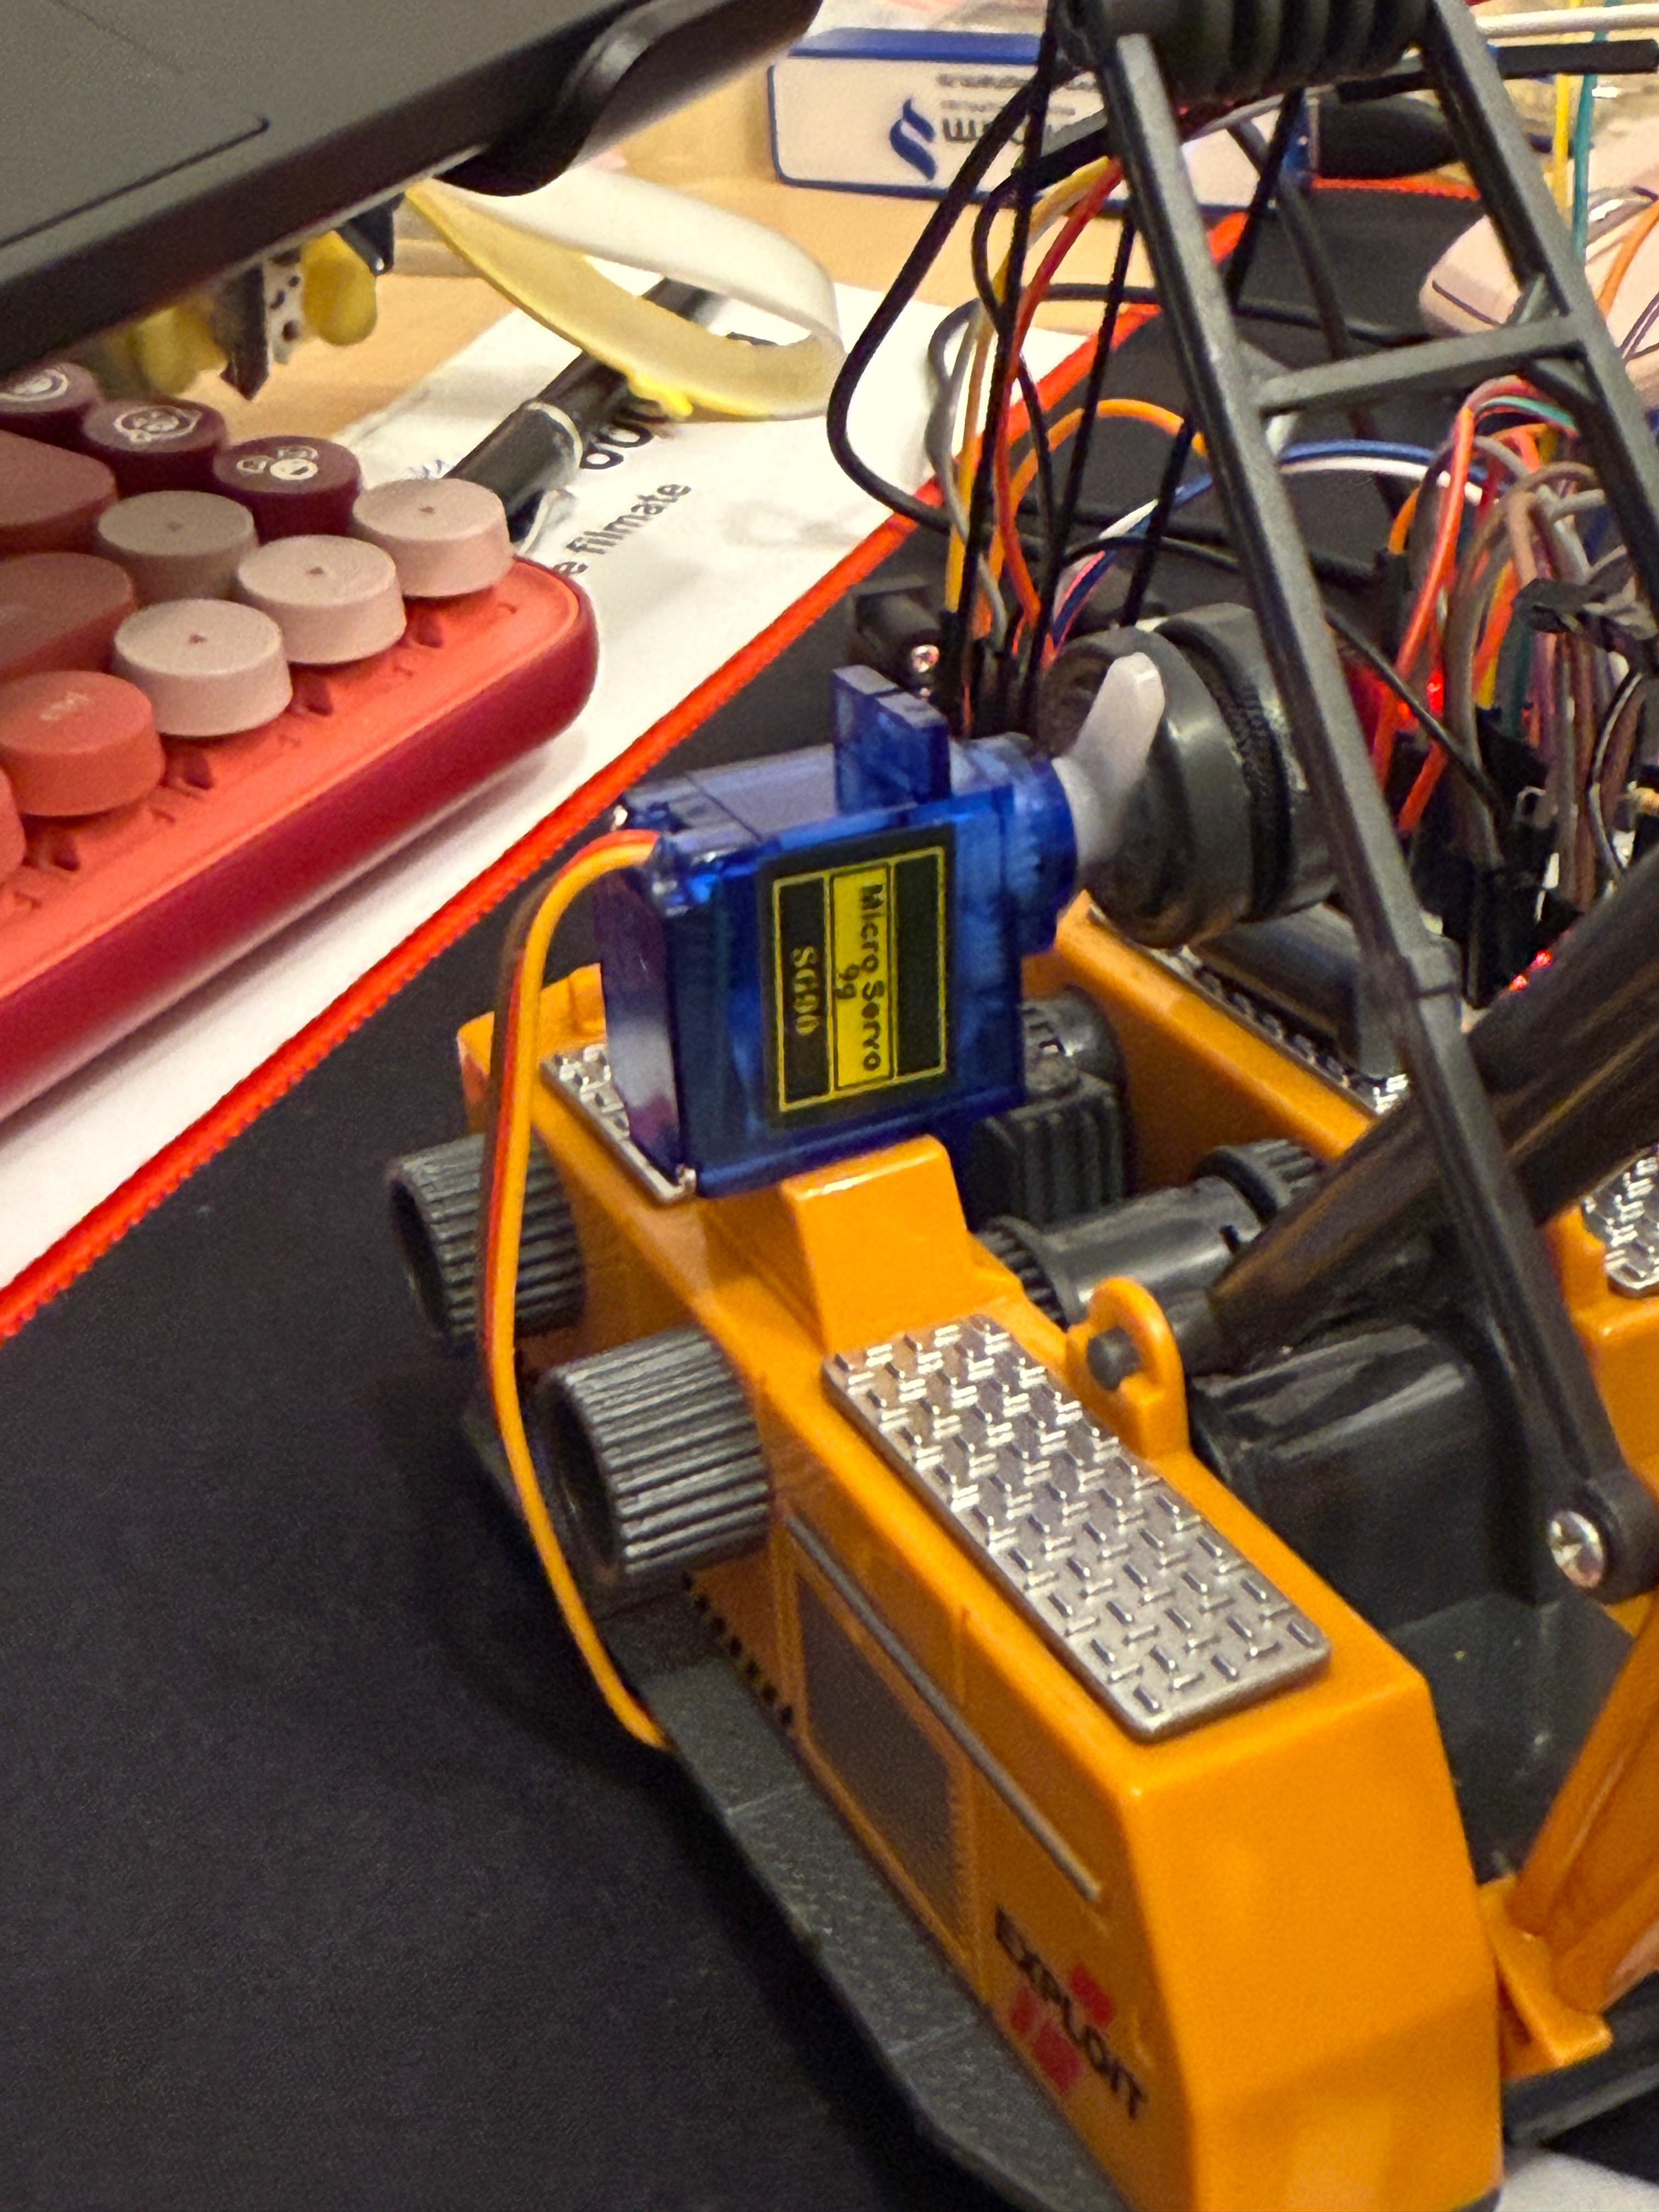
\includegraphics[width=\textwidth]{figures/4.jpg}
      \caption{Servomotor}
  \end{subfigure}
  \hfill
  \begin{subfigure}[b]{0.3\textwidth} % 5-a imagine
      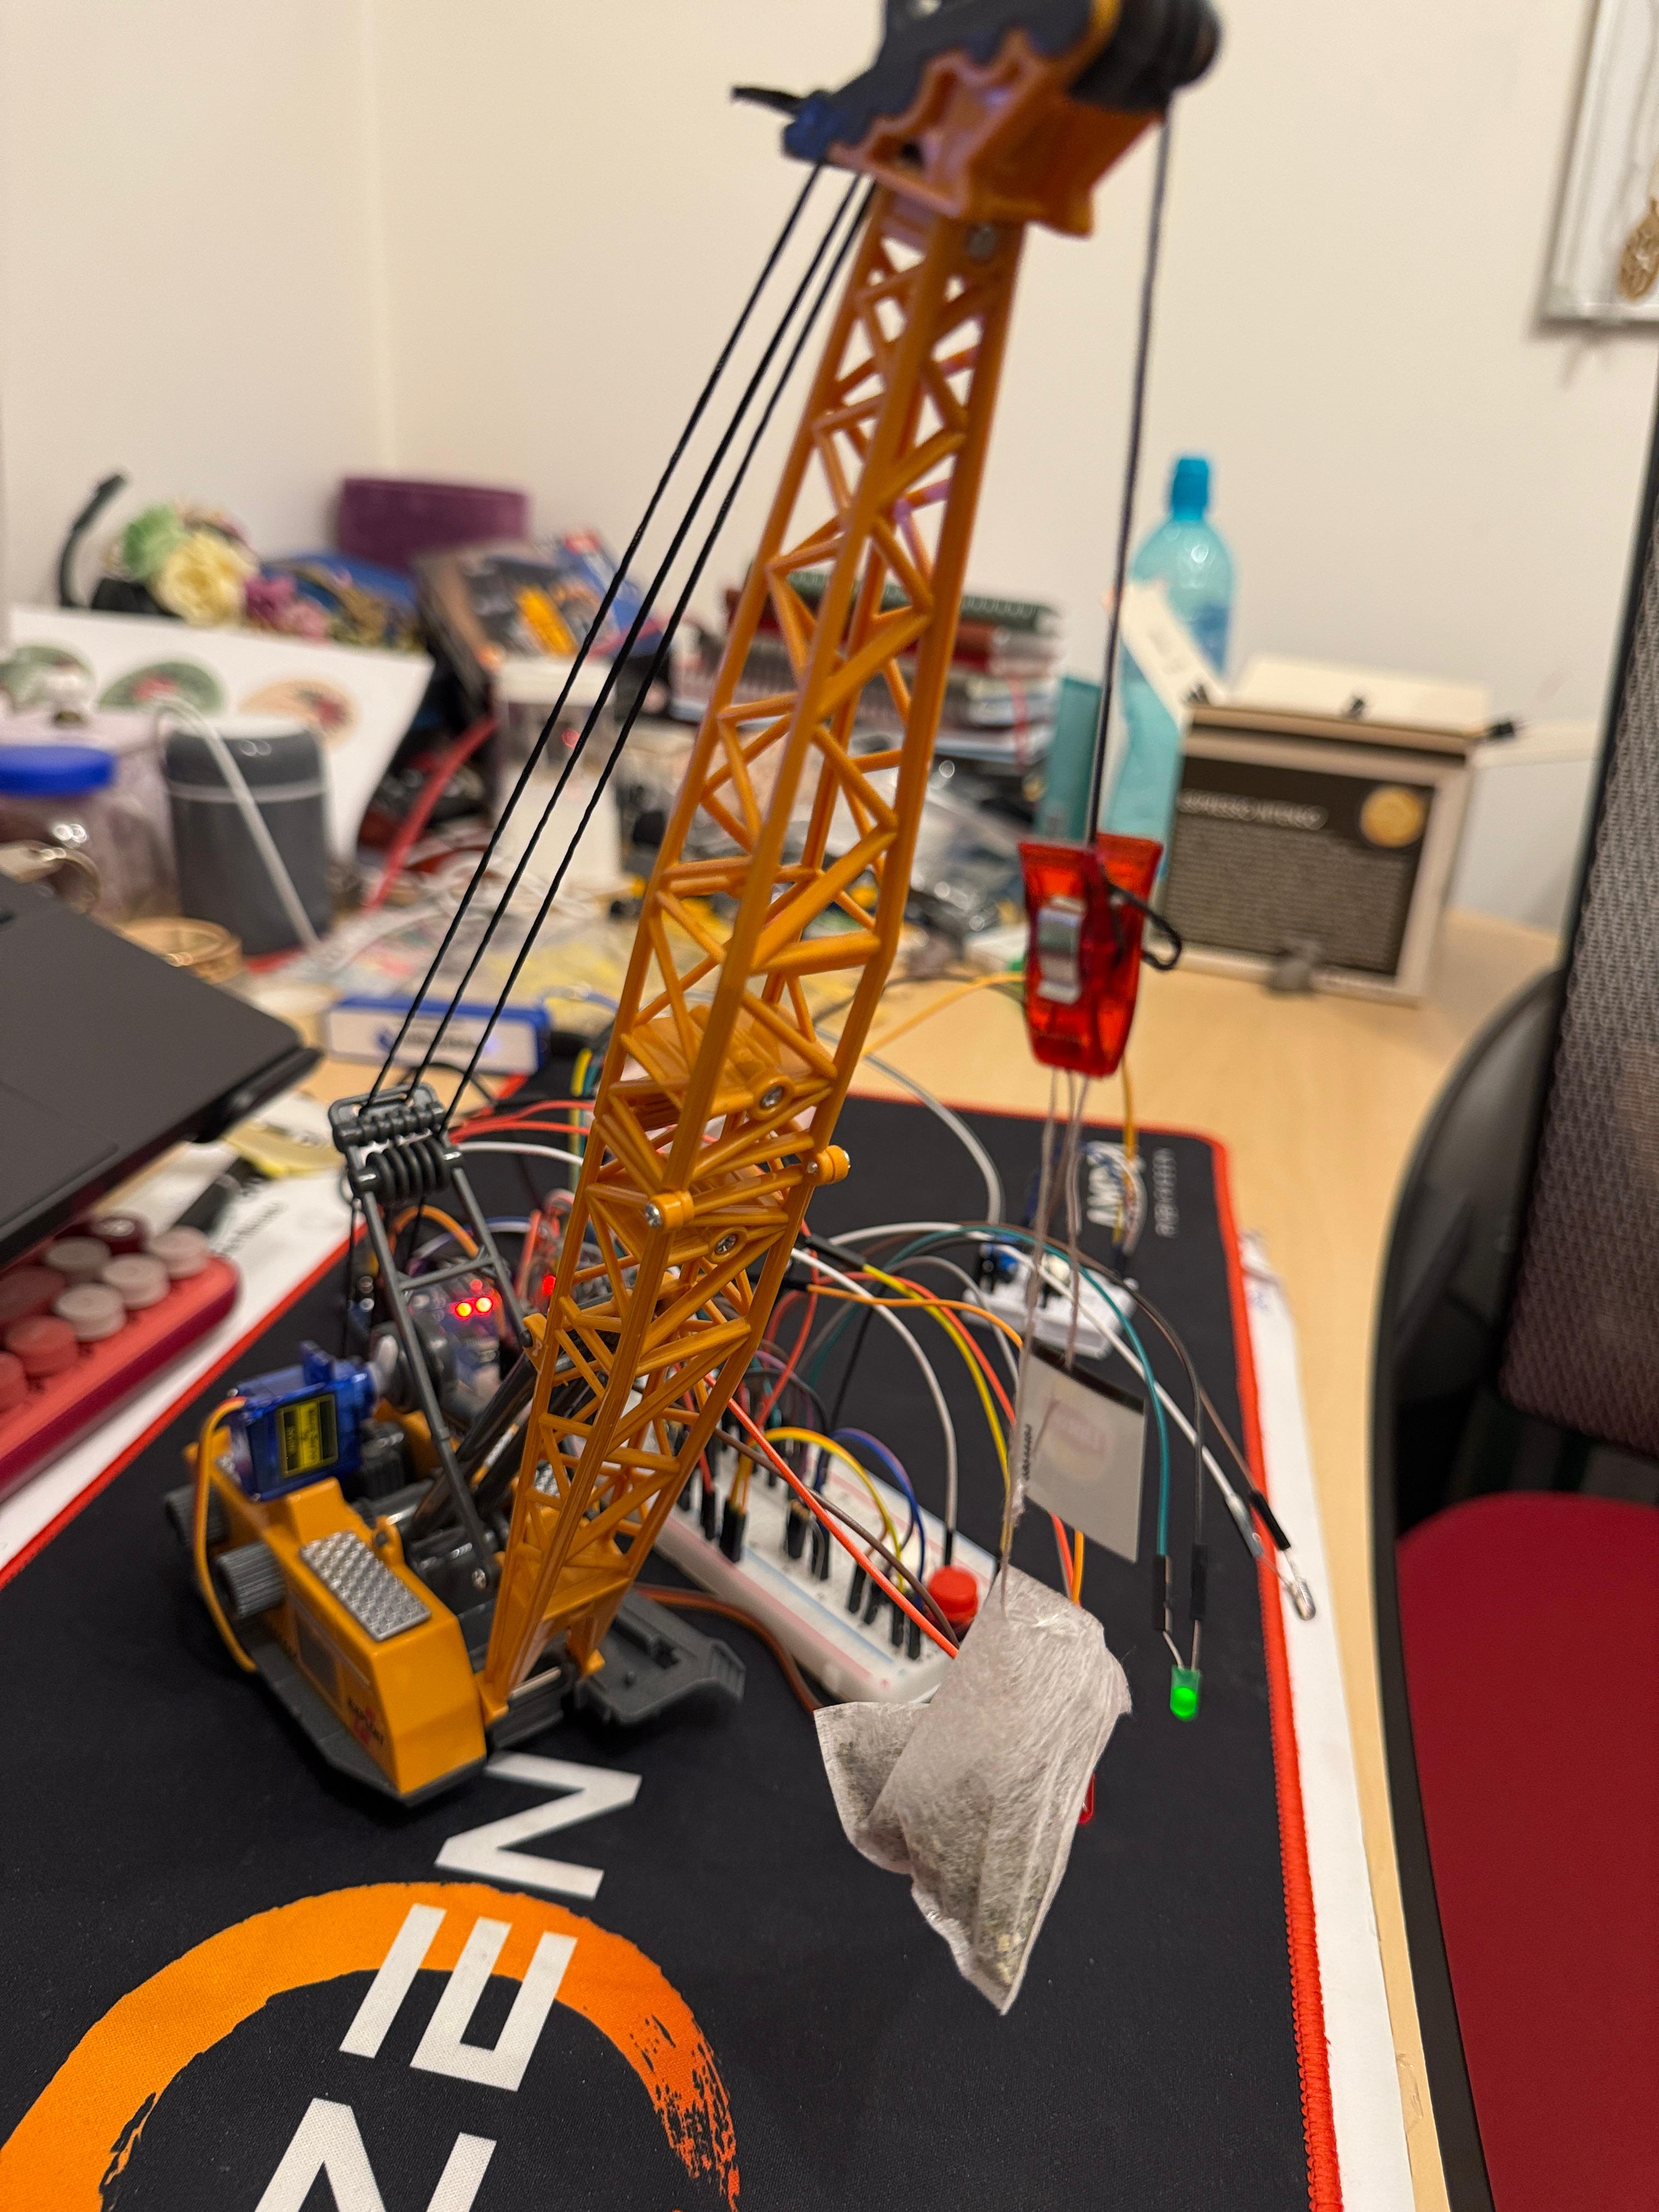
\includegraphics[width=\textwidth]{figures/5.jpg}
      \caption{Macara de jucărie}
  \end{subfigure}

  \caption{Componente și Conexiuni}
  \label{fig:matrice_imagini}
\end{figure}

\begin{figure}[ht!]
  \centering
  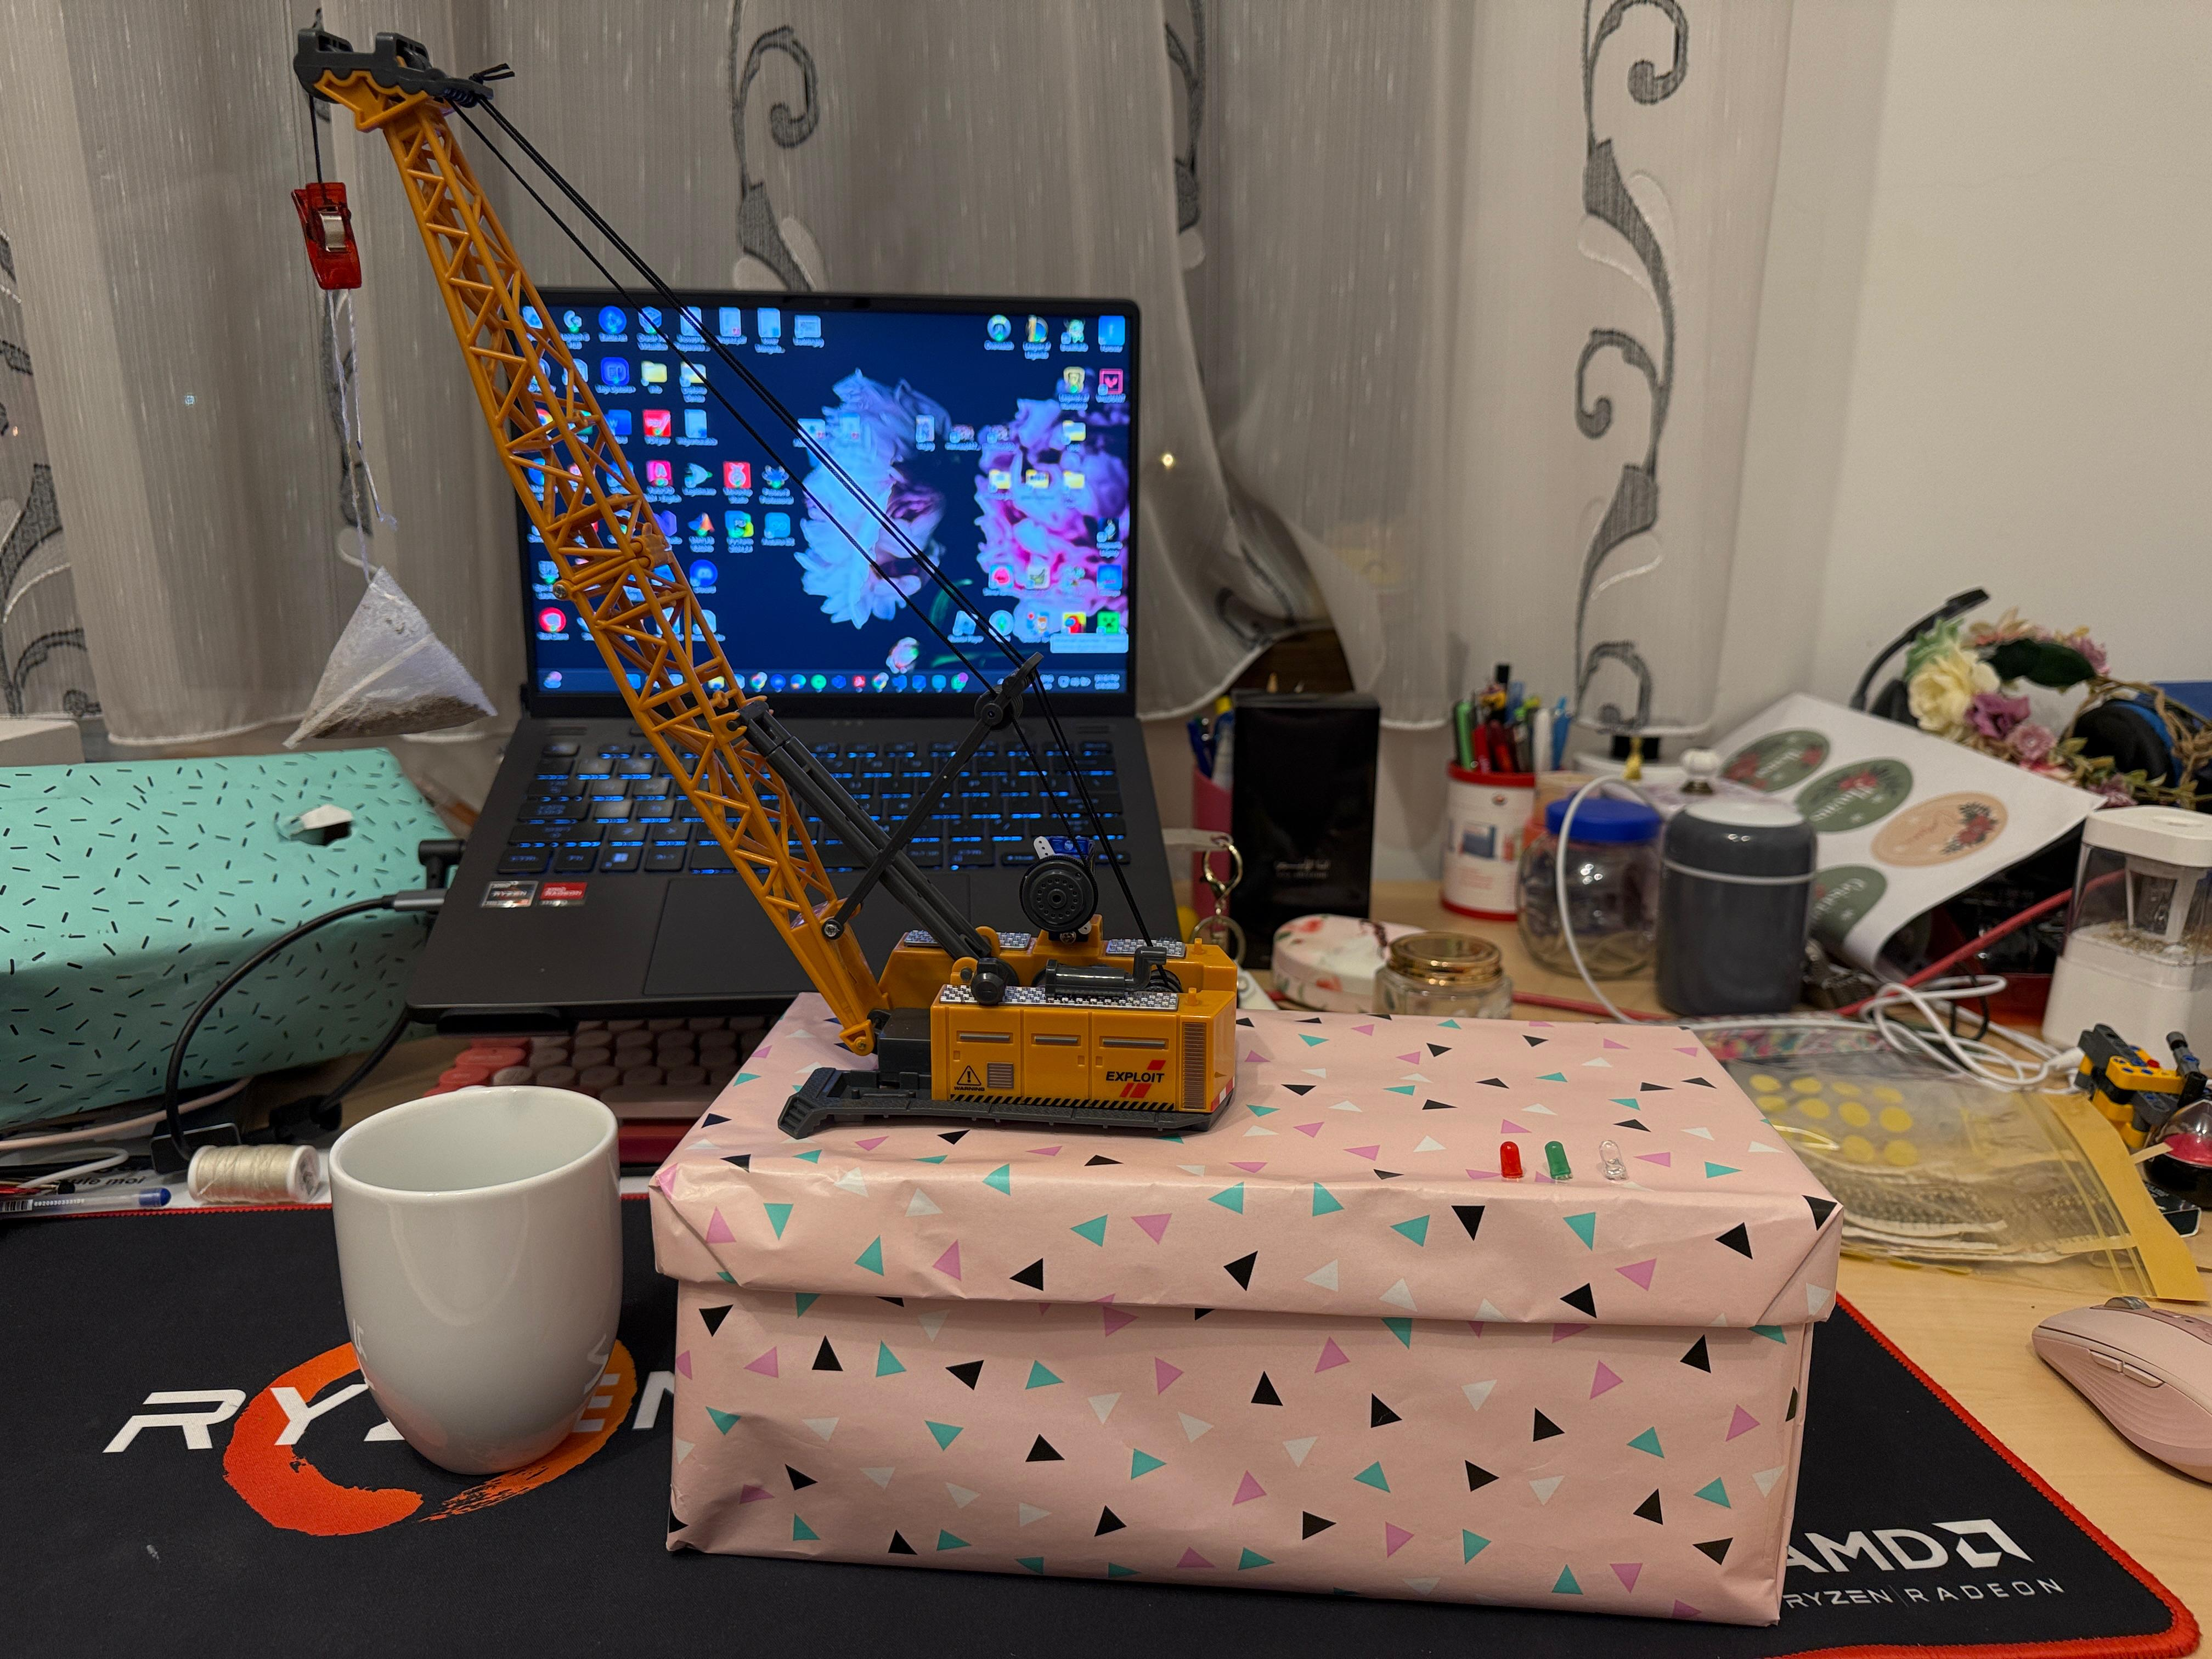
\includegraphics[width=\textwidth]{figures/6.jpg} 
  \caption{Asamblarea Finală}
  \label{fig:fig4}
\end{figure}
\addcontentsline{toc}{chapter}{\protect Lista de Figuri}
\listoffigures






\end{document}